\documentclass[11pt]{article}

\usepackage[margin=1.15in]{geometry}
\usepackage{amsmath,amssymb,amsthm}
\usepackage{graphicx}
\usepackage{booktabs}
\usepackage{xcolor}
\usepackage[round]{natbib}
\usepackage[colorlinks=true,linkcolor=blue!60!black,citecolor=blue!60!black,urlcolor=blue!60!black]{hyperref}
\usepackage{microtype}

% ---------- theorem environments ----------
\newtheorem{theorem}{Theorem}
\newtheorem{proposition}{Proposition}
\newtheorem{lemma}{Lemma}[section]
\newtheorem{corollary}{Corollary}[section]
\newtheorem{conjecture}{Conjecture}
\newtheorem{observation}{Observation}
\newtheorem*{restatedproposition}{Restatement}
\newtheorem*{restatedconjecture}{Restatement}
\newtheorem*{restatedobservation}{Restatement}
\theoremstyle{definition}
\newtheorem{assumption}{Assumption}
\theoremstyle{remark}
\newtheorem{remark}{Remark}[section]

% Manual-tag assumption blocks used inside appendix proofs (drafts carry
% their own per-proposition assumption labels A1..An).
\newenvironment{assumptionlist}{\begin{description}}{\end{description}}

\newcommand{\pim}{\pi_{\mathrm{m}}}
\newcommand{\pir}{\pi_{\mathrm{r}}}
\newcommand{\popp}{p_{\mathrm{opp}}}
\newcommand{\ktype}{k_{\mathrm{type}}}
\newcommand{\kpiv}{k_{\mathrm{piv}}}

\title{Clearing Conditional Commitments:\\
\large Privacy, Specification, and Custody in a Clearinghouse for Interdependent Action\thanks{%
Preliminary working draft (v1, June 2026). Comments welcome. The numerical companion --- a
chain of nine verified ``toy model'' memos, the solver scripts, and the adversarial
verification logs --- is available from the author. All errors are mine.}}
\author{Timothy J. Miano\thanks{Affiliate, Massachusetts Institute of Technology; and Founder \& CEO, Proffer Futures, Inc. Contact: \texttt{timmiano@mit.edu}. \emph{Disclosure:} the author holds equity in Proffer Futures, Inc., which operates the ifwishlist platform discussed in Section~9.}}
\date{June 2026 --- preliminary and incomplete}

\begin{document}
\maketitle

\begin{abstract}
\noindent
Latent willingness of the form ``I will, if enough of the right others will'' has no
standard clearing institution. We model a \emph{conditional-commitment clearinghouse}: a platform
that authenticates participants (accuracy $q$), verifies that their mutual conditions are
jointly satisfiable (consensus integrity $c$), routes compatible counterparts to one another,
and chooses three design dials --- custody of principal $\gamma$, specification timing
$\sigma$, and disclosure granularity $k$ --- before activating the coalition at a fixed
point. Our central result is that the welfare-maximizing clearinghouse is \emph{minimal on
all three dials at once}: it holds no principal, fixes terms late, and discloses progress
only through a $k$-anonymized aggregate. The result is stated with its boundary: it holds in
a bounded high-authenticity, intermediate-integrity region, reverses on each axis outside
it, and the three minimalisms are coupled in welfare magnitude rather than additively
separable. Three further results discipline the disclosure claim. First, the privacy dial's
screening cost is a genuine information-leakage object --- the Shannon mutual information
between coalition type and the $k$-anonymized support count --- and full disclosure does not
perfectly screen. Second, the masking advantage survives a refinement-free selection: under
Carlsson--van~Damme risk dominance no rationality parameter appears anywhere in the
model, the revealed game's contested-regime collapse is exact, and masked momentum is
sustained --- proven at the deadline rung and for the smallest coalitions, conjecture-gated
(and grid-verified) at interior rungs. Third, partial
masking is \emph{constrained-optimal for a structural reason}: a single disclosure dial
necessarily bundles ``this coalition is real'' with ``you are not pivotal,'' so --- in a
one-round theorem extended by a dynamic calibration --- the interior optimum exists even
where the unconstrained ideal would be full type-disclosure with zero pivotality leakage. We state three formal propositions with complete proofs, enumerate the
open conjectures, and propose an administrable safe-harbor rule keyed to the mechanism's
structure.\\[4pt]
\textbf{JEL:} C72, D82, D47, H41.\quad
\textbf{Keywords:} conditional commitment, coordination, information design, $k$-anonymity,
market design, assurance contracts.
\end{abstract}

% =====================================================================
\section{Introduction}\label{sec:intro}

\subsection{The vocabulary, fixed first}

The broad problem family is \emph{interdependent action}: situations where each
participant's willingness to act depends on who else will act, in what number, under what
terms, and with what visibility. Collective action, collective consumption, assurance,
focal-point coordination, and matching and scheduling are subcases --- the family is broad,
and we will not pretend any one branch is the genus.

The economic object this paper introduces is the \emph{conditional commitment}: ``I will,
if a qualifying composition of others will.'' Not a pledge (a scalar added to a total), but
a node with edges --- a private commitment whose condition refers to the \emph{composition}
of the committing set: rosters, roles, types, compound thresholds.

The institution that makes the object clearable is the \emph{conditional-commitment
clearinghouse}: private conditional commitments are collected, checked for joint
satisfiability, and activated at the moment the edge-constraints are simultaneously
satisfied --- a fixed point whose output is common knowledge of a feasible coalition. It
clears commitments, not prices. Markets clear goods; this institution clears conditional
commitments --- and in doing so makes previously unclearable interdependent action
actionable.

\subsection{The friction: why the clearinghouse never existed}

Conditional willingness has always existed. No institution cleared it because four barriers
stood at once, and removing any three does not open the institution:
credibility (``I would'' is cheap talk; signals are forgeable), compatibility (mutual
conditions may not be jointly satisfiable --- is there a real coalition, or sixty unrelated
``ifs''?), discoverability (compatible counterparts cannot find each other), and legality
(turning activation into value movement can trigger custody, transmission, or liability
regimes). The institution's non-existence was overdetermined: each wall alone is fatal. The
thesis is that the four walls are now jointly removable for the first time --- credibility
and discoverability by algorithmic inference at scale, compatibility by a mechanism-design
move, legality by a legal-architecture move.

\subsection{The contribution}

Three results, in increasing order of surprise.

\emph{First, a clearable primitive.} We formalize the conditional commitment as a graph
object --- nodes, compositional edge-constraints, a fixed-point activation event --- and
show that a pledge-threshold mechanism is its scalar degenerate case
(Section~\ref{sec:model}).

\emph{Second, one central result, three minimalisms.} In a single welfare objective over custody
$\gamma$, specification $\sigma$, and disclosure $k$, the joint optimum is the minimal
corner on all three axes together --- no custody, fuzzy-early specification, partial
masking --- in a bounded high-$q$, intermediate-$c$ region, reversing off it on each axis
(Section~\ref{sec:central}). The efficient clearinghouse clears \emph{because} it
withholds.

\emph{Third, the disclosure dial decomposed.} The privacy dial controls two channels with
opposite signs --- type/screening (favoring disclosure) and pivotality/protection (favoring
masking) --- and because one physical dial bundles them, partial masking is
constrained-optimal even where the unconstrained ideal is full type-disclosure
(Sections~\ref{sec:dial}--\ref{sec:selection}). The screening cost of masking is quantified
by an actual information measure, and the protection advantage survives a refinement-free
equilibrium selection (with the momentum bound conjecture-gated at interior rungs, as the
proposition statement discloses). Proposition~\ref{prop:band} establishes the interior masking band in
integrity; Proposition~\ref{prop:selection} the refinement-free selection;
Proposition~\ref{prop:bundle} the bundled-dial structure of partial masking.

The displacement claim in one line: prior work either fixes the good, conditions on a sum,
or treats common knowledge as exogenous; we endogenize the good, the coalition membership,
and the disclosure boundary, and then clear relational conditional commitments.

% =====================================================================
\section{Related literature}\label{sec:lit}

Six lineages bracket the contribution; none contains it.

\paragraph{Collective action and provision points.}
\citet{olson1965logic} names the free-rider problem but offers no clearing institution.
\citet{bagnoli1989provision} and the assurance-contract mechanisms of
\citet{tabarrok1998private} fix the good ex ante and condition on a \emph{scalar}
threshold; we endogenize the good's terms and make the condition \emph{relational}
(compositional edge-constraints). \citet{marxmatthews2000dynamic} is the direct dynamic
ancestor --- an observable running total as the Markov coordinating state in voluntary
contribution --- and supplies the completion structure, but contains no disclosure-design
result. \citet{halac2020raising} reach unique implementation through contingent
\emph{payments} to heterogeneous investors over a scalar threshold: the transfer route to
the destination our disclosure route reaches.

\paragraph{Coordination and common knowledge.}
Schelling's focal points and \citet{chwe2001rational} explain when coordination succeeds
given common knowledge; we \emph{manufacture} common knowledge as a service, with
endogenous membership. The global-games selection machinery we draw on is
\citet{carlsson1993global} and \citet{frankelmorrispauzner2003equilibrium}. We cite the
latter's \S6.4 for the criterion's pedigree, not as a blanket license: where the stage game
has strategic complementarities, their \S6.4/Theorem~4 identifies the Laplacian
(uniform-belief) action as the noise-independent selection; at the pivotal (diagonal)
states that drive our result the stage game is a volunteer's dilemma --- commit and wait
are strategic \emph{substitutes} there --- which falls outside the licensed class, so at
those states we adopt the Laplacian action as the \emph{definition} of stagewise risk
dominance, cross-validated by an independent $\lambda$-free potential-maximizer refinement
(Proposition~\ref{prop:selection} and its Appendix~\ref{app:P2} scoping).

\paragraph{Information design.}
\citet{morris2002social} and \citet{cornand2008publicity} establish that public disclosure
precision can flip welfare; \citet{li2023global} studies obfuscation directly. In all
three, precision is a Gaussian noise parameter on a fundamental --- not a quantified
privacy-mechanism leakage measure, and there is no coalition screening rate.
\citet{kamenica2011bayesian}, \citet{bergemann2019information},
\citet{morris2024implementation}, and \citet{inostroza2025adversarial} supply the
persuasion, BCE, and adversarial-selection toolkit over payoff states: lineage, not
preemption. \citet{vosooghi2017information} is nearest by setting --- information design
inside coalition formation --- but the lever is beliefs about a scalar social-cost state,
not a privacy mechanism; its published dynamic extension
\citep{vosooghi2022information} has a third-party sender choosing threshold revelation of
a scalar fundamental to a single coalition, with no privacy mechanism over participant
structure and no screening rate. \citet{halac2021rank} is the closest
privacy-as-instrument neighbor (rank uncertainty defeating strategic uncertainty in team
production), with no quantified leakage primitive. \citet{chen2023stability} is the
matching-side precedent for stability being information-structure-relative, with pairwise
types and no disclosure welfare sign-flip.

\paragraph{Crowdfunding and matching.} The crowdfunding design literature
\citep{strausz2017crowdfunding,ellman2019optimal,belleflamme2014crowdfunding} studies
all-or-nothing thresholds and moral hazard over a \emph{fixed} good with a scalar target;
matching with contracts \citep{hatfield2005matching} clears relational structure but over
fixed contract terms with no disclosure design. Both condition on what we endogenize.

\paragraph{Market design.}
The program of \citet{roth1999redesign,roth2002engineer} --- designing clearing
institutions for market-like environments that did not previously clear --- is the lineage
we claim membership in. \citet{weyl2018radical} is nearest in ambition, distinct in
object: we clear non-transferable conditional commitments, not assets or votes.

\paragraph{The new ingredient,} absent from each lineage by construction, is a
\emph{quantified privacy-leakage primitive} (the mutual information between coalition type
and a $k$-anonymized support count) \emph{driving a coalition screening rate}, joined to a
difficulty-keyed masking advantage. That conjunction is the contribution.

% =====================================================================
\section{The environment}\label{sec:model}

$N$ agents; one latent outcome whose terms are not yet fixed. Each agent $i$ holds a
private type and a conditional commitment $c_i = $ ``act if composition $S_i$ of others
commits.'' A resolver authenticates nodes with accuracy $q$. A router surfaces the outcome
to compatible agents. Coalitions are of two types, good (deliverable) and bad (illusory),
with prior $\pi_b$ on bad; consensus integrity $c$ indexes the probability that the posted
conditional structure is jointly satisfiable.

The platform chooses three dials:
\begin{itemize}
\item \textbf{Custody} $\gamma \in [0,1]$ --- the fraction of principal held at commitment
time, carrying a trust-liability cost $c_{\mathrm{cust}}\gamma$ and deadweight $d_\gamma$,
against a possible commitment-device benefit $\beta_\gamma$ that can lower the effective
activation cutoff.
\item \textbf{Specification} $\sigma \in [0,1]$ --- how early the outcome's terms harden.
Precise-early kills latent commitments via the compatibility factor
$\mathrm{comp}(\sigma)$; fuzzy-too-long adds indeterminacy cost $\mathrm{indet}(\sigma)$.
The outcome's terms may be an \emph{endogenous output} co-resolved by the committed set:
scheduling-by-coalition is the clean instance, where the date is selected by the coalition
rather than fixed before the coalition exists.
\item \textbf{Disclosure} $k \in [0,1]$ --- the granularity of progress disclosure,
implemented as a $k$-anonymity dial on the support count (additive blur
$r(k) = \mathrm{round}((1-k)N)$).
\end{itemize}

Activation occurs when the edge-constraints are simultaneously satisfiable --- the fixed
point --- after which campaign terms harden and value, where present, moves on the
recipient's own rail (the platform holds nothing). The welfare objective of the unified
numerical model is
\begin{equation}\label{eq:W}
W(\gamma,\sigma,k;\,q,c) \;=\;
\mathrm{comp}(\sigma)\,\bigl(1-\rho_{\mathrm{eff}}(k,\gamma,c)\bigr)\,
\bigl(V-\mathrm{indet}(\sigma)\bigr)\,(1-d_\gamma\gamma)
\;-\;\bigl(1-\mathrm{comp}(\sigma)\bigr)\bigl(1-s(k)\bigr)L
\;-\;c_{\mathrm{cust}}\gamma,
\end{equation}
where $\rho_{\mathrm{eff}}$ is the effective unraveling risk and $s(k)$ the bad-coalition
screening rate. We solve for when an activatable coalition forms --- the fixed point exists
\emph{and is selected} --- and for the dial setting that maximizes welfare: coalitions that
should form, do; spurious ones do not.

\paragraph{Reduced-form status.} The unified objective \eqref{eq:W}, the revealed game's
pivotality blend, and the bundled-dial channel coupling are disciplined reduced-form
primitives, not objects derived from a Bayesian extensive form; the appendices state this
where each is used, and each appendix's local model is self-contained (local symbols are
local). The conclusions most robust to this level of abstraction are the structural ones
--- the two-channel decomposition, the bundling constraint, the regime splits; the
quantitative surfaces are measurement targets (Section~\ref{sec:empirics}).

% =====================================================================
\section{The central result: minimal is optimal}\label{sec:central}

\begin{theorem}[informal; numerically established]\label{thm:minimal}
In a bounded high-authenticity, intermediate-integrity region, and under a bounded
custody-benefit, the welfare-maximizing clearinghouse reduces custody, specification, and
disclosure together: the joint optimum $(\gamma^*,\sigma^*,k^*)$ of \eqref{eq:W} is
$\gamma^*=0$ (no custody), $\sigma^*=0$ (fuzzy-early), and $k^*<1$ (partial masking). The
optimum reverses off the region on each axis. The three dials are coupled in welfare
magnitude --- quasi-separable in threshold structure, not additively separable --- with
specification$\times$disclosure the leading interaction.
\end{theorem}

Each apparent weakness does real work. The clearinghouse clears precisely because it
withholds: holding principal adds a trust liability the clearing does not require; forcing
terms early kills latent commitments before the coalition can form; revealing granular
pivotal state can unravel the conditional consensus it is meant to advertise.

Theorem~\ref{thm:minimal} is established numerically (a restricted static disclosure facet
is the part proven analytically, as Proposition~\ref{prop:band} below); four qualifiers travel with
it. \emph{Region, not everywhere}: the joint-all-minimal bands are $c\in[0.66,0.72]$ at
$q=0.95$ and $c\in[0.64,0.74]$ at $q=1.0$, and the region requires $q \gtrsim 0.95$; the
masking band in $c$ is an interior band --- transparency wins below it (screening
dominates) and, for $q<1$, above it (at $q=1$ with the reference parameters the upper
closure fails and masking persists toward $c=1$, Appendix~\ref{app:P1}). \emph{Coupled, not separable}:
the three-dimensional joint argmax equals the product of one-dimensional argmaxes in only
221 of 600 parameter draws; the welfare cost of the separable policy is typically small
(median $0.43\%$) with a real tail ($p_{95}=92\%$). \emph{Custody-minimalism is the
bounded claim}: $\gamma^*=0$ holds only when the commitment-device benefit is small
($\beta_\gamma \ge 0.25$ flips it), the qualifier \citet{diamond1984delegated} already
suggests. \emph{Minimal disclosure means partial masking}: the optimal dial is an interior
$k$-anonymity level, not a blackout; and the \emph{dynamic} (live progress-bar) version of
the masking advantage is a finite-$N$ effect that vanishes in the continuum --- the durable
large-population result is the static coordination/screening logic. The dynamic effect is
real for small campaigns, which is the regime the live platform actually runs.

% =====================================================================
\section{The disclosure dial decomposed}\label{sec:dial}

The single dial $k$ controls two information channels with opposite signs.

\subsection{The type/screening channel}

Disclosure carries a signal about coalition \emph{type} --- good (deliverable) versus bad
(illusory). The channel's precision is grounded in an actual information measure: the
support count $m \sim \mathrm{Binom}(N, p_\psi)$ with $p_G > p_B$ is published under
$k$-anonymity, and precision is the Shannon mutual information $I(\text{type};
m_{\mathrm{obs}})$. The numerical findings, each surviving cross-mechanism
re-implementation: $I(k)$ is monotone (data processing) and \emph{saturating}
($I(1)=0.62$ bits $< H=0.97$ at the reference calibration --- the exact count does not
perfectly reveal type, because the binomial supports overlap); therefore full disclosure
does not perfectly screen, $s(1)<1$, \emph{derived} from the support gap rather than
posited, with $s(1)\to1$ recovered in the large-gap perfect-separation limit; and the
screening rate $s(k)$ is non-monotone under a pessimistic prior. One scope restriction: at
$k=1$ every privacy mechanism collapses to the exact count, so the endpoint is pinned by
$(p_G,p_B)$ alone, and the curve's interior shape is mechanism-dependent. The grounding
closes the endpoint, not the curve; $(p_G,p_B)$ is itself the next-deeper primitive.

\subsection{The pivotality/protection channel}

Disclosure also reveals \emph{pivotal structure} --- who is and is not needed. The two
channels live in complementary excludability regimes: the type channel has bite only at
$\xi < 1-\kappa/V$, where the activation payoff exceeds the free-ride payoff; the
protection channel operates in the complementary regime where free-riding pays
($\xi > 1-\kappa/V$). There, in a contested market, revealing pivotality lets
inframarginal movers free-ride and collapses clearing; masking forces every committer to
act as if pivotal, sustaining the coalition.

\subsection{The static band: a theorem}

The static interplay of screening and unraveling produces the central disclosure
comparative static: partial masking is optimal on a nonempty set contained strictly inside
the interior of the integrity range --- a single band in every tested calibration, with
connectedness the one open conjecture. Figure~\ref{fig:band} displays it; Proposition~\ref{prop:band} proves it.

\begin{figure}[t]
\centering
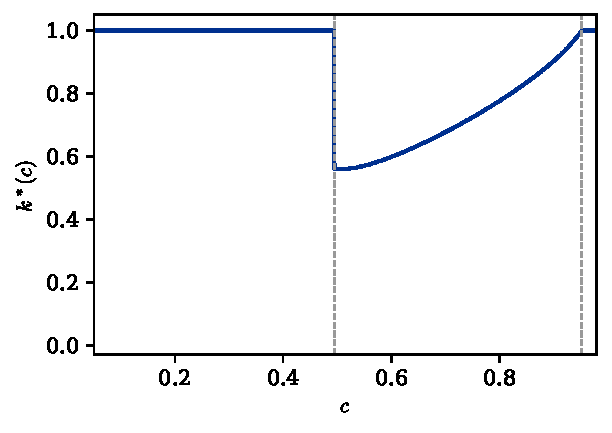
\includegraphics[width=0.62\textwidth]{figures/fig-band.pdf}
\caption{The interior masking band. Optimal disclosure $k^*(c)$ in the static model at
$q=0.95$ ($V=1$, $L=1.2$, $\tau=0.7$, Beta integrity family with concentration $\eta=8$).
Full disclosure is optimal at both integrity extremes; partial masking on the interior
band (dashed edges). The lower transition is a discontinuous global-max switch; the upper
transition is continuous (Appendix~\ref{app:P1}).}
\label{fig:band}
\end{figure}

% ---------------------------------------------------------------------------
% P1-statement.tex --- formal statement of Proposition \ref{prop:band}
% (interior masking band in consensus integrity). Proof: appendix/P1-proof.tex.
% Converted from docs/propositions-workdir/P1-draft.md (content frozen;
% notation renames only: kappa -> eta, theta -> r per the paper's canon).
% ---------------------------------------------------------------------------

The platform chooses a disclosure granularity $k \in [0,1]$ ($k = 1$ full disclosure,
$k = 0$ full masking). A coalition is good with probability $qc$ and bad with
probability $1 - qc$, where $q \in (0,1]$ is authentication accuracy and $c \in (0,1)$
is consensus integrity. A good coalition has robustness $r_g \sim F_c$ on $[0,1]$ and
delivers surplus $V > 0$ unless it unravels, which occurs iff $r_g < \hat r(k)$, where
$\hat r(k)$ is the strategic activation cutoff induced by disclosure level $k$; a bad
coalition imposes loss $L > 0$ unless screened, which happens with probability $s(k)$.
Welfare is
\begin{equation}
W(k; q, c) \;=\; qcV\bigl(1 - F_c(\tau k)\bigr) \;-\; (1 - qc)\,L\,(1 - k).
\tag{W}\label{eq:Wband}
\end{equation}
Let $K^*(c) := \operatorname*{arg\,max}_{k \in [0,1]} W(k; q, c)$ (the dependence on
$q$ is suppressed except in part~(e)). We write ``full disclosure is uniquely optimal
at $c$'' for $K^*(c) = \{1\}$ and ``masking is optimal at $c$'' for $1 \notin K^*(c)$.
Define the \emph{masking set}
\[
M \;:=\; \{\, c \in (0,1) : 1 \notin K^*(c) \,\},
\]
and the \emph{marginal-balance function} (minus the right-hand slope of $W$ at $k = 1$)
\begin{equation}
\varphi(c) \;:=\; qcV\tau f_c(\tau) \;-\; (1 - qc)\,L.
\tag{$\varphi$}\label{eq:phi}
\end{equation}
$\varphi(c) > 0$ says: at full disclosure, the marginal unraveling loss
$qcV\tau f_c(\tau)$ exceeds the marginal screening gain $(1 - qc)L$.

\begin{assumption}\label{ass:band}
\leavevmode
\begin{itemize}
\item[\textbf{(A1)}] \textbf{(Payoffs.)} $V, L > 0$, $\tau \in (0,1)$, $q \in (0,1]$,
  $c \in (0,1)$; welfare is \eqref{eq:Wband}.
\item[\textbf{(A2)}] \textbf{(Linear channels --- restriction.)} $\hat r(k) = \tau k$,
  $s(k) = k$, hence the unraveling risk is $\rho(k,c) = F_c(\tau k)$. This is exactly
  the specification of the numerical ground-truth scripts \texttt{v3.py}~/
  \texttt{v3\_shape.py}.
\item[\textbf{(A3)}] \textbf{(Family regularity.)} For each $c \in (0,1)$, $F_c$ is a
  CDF on $[0,1]$ with density $f_c$ strictly positive and continuous on $(0,1)$, and
  $(r, c) \mapsto f_c(r)$ is continuous on $(0,1) \times (0,1)$.
\item[\textbf{(A4)}] \textbf{(Fragile-end thinness at the cutoff.)} There exists
  $\bar k \in (0,1)$ with
  \[
  \lim_{c \to 0^+} \; c \, \sup_{r \in [\tau\bar k,\, \tau]} f_c(r) \;=\; 0.
  \]
  (At very low integrity, the robustness density of good coalitions carries vanishing
  $c$-weighted mass near the transparency cutoff $\tau$.)
\item[\textbf{(A5)}] \textbf{(Robust-end thinness below the cutoff.)}
  {\sloppy
  $\lim_{c \to 1^-} S(c) = 0$, where $S(c) := \sup_{r \in (0,\tau]} f_c(r)$, and
  \textbf{either} (i) $q < 1$, \textbf{or} (ii)
  \[
  \limsup_{c \to 1^-} \; \frac{cV\tau S(c)}{(1 - c)L} \;<\; 1.
  \]
  (At very high integrity, good coalitions are too robust to unravel: the density on
  $[0, \tau]$ vanishes --- fast enough, relative to $1 - c$, if $q = 1$.)\par}
\item[\textbf{(A6)}] \textbf{(Interior bite --- non-vacuity.)} There exists
  $c_m \in (0,1)$ with $\varphi(c_m) > 0$, i.e.
  \[
  q\, c_m V \tau f_{c_m}(\tau) \;>\; (1 - q c_m)\, L.
  \]
\item[\textbf{(A7)}] \textbf{(Beta specialization, for parts (d).)}
  $F_c = \mathrm{Beta}\bigl(c\eta, (1-c)\eta\bigr)$ on $[0,1]$ with fixed concentration
  $\eta > 2$ (mean $c$; the family of v2/v3 and of \texttt{v3\_shape.py}). Define
  \[
  \bar c \;:=\; \frac{1 + \tau(\eta - 2)}{\eta} \;\in\; \Bigl(\frac{1}{\eta},\, 1\Bigr)
  \qquad \text{(the concavity threshold)},
  \]
  the smallest $c$ at which the Beta mode $(c\eta - 1)/(\eta - 2)$ reaches $\tau$.
\end{itemize}
\end{assumption}

\begin{proposition}[Interior masking band in $c$]\label{prop:band}
Assume A1--A3.
\begin{itemize}
\item[\textup{(a)}] \textup{(Existence.)} For every $c \in (0,1)$, $W(\cdot\,; c)$ is
continuous on $[0,1]$ and $K^*(c) \neq \emptyset$.
\end{itemize}
Assume in addition A4--A6. Then:
\begin{itemize}
\item[\textup{(b)}] \textup{(Full disclosure at both extremes.)} There exist
$0 < c_1 \le c_2 < 1$ such that $K^*(c) = \{1\}$ for every $c \in (0, c_1)$ and every
$c \in (c_2, 1)$.
\item[\textup{(c)}] \textup{(Masking in the middle; the band.)} $1 \notin K^*(c_m)$, so
$M \neq \emptyset$. Consequently
\[
c_{\mathrm{lo}} := \inf M \quad\text{and}\quad c_{\mathrm{hi}} := \sup M
\]
satisfy $0 < c_1 \le c_{\mathrm{lo}} \le c_m \le c_{\mathrm{hi}} \le c_2 < 1$; full
disclosure is optimal ($1 \in K^*(c)$) for every
$c \in (0, c_{\mathrm{lo}}) \cup (c_{\mathrm{hi}}, 1)$, uniquely so on
$(0, c_1) \cup (c_2, 1)$; and masking is strictly optimal at
$c_m \in [c_{\mathrm{lo}}, c_{\mathrm{hi}}]$. In particular the masking region is
contained in a band strictly interior to $(0,1)$ and is nonempty.
\end{itemize}
Assume in addition A7. Then:
\begin{itemize}
\item[\textup{(d)}] \textup{(Sharp upper threshold and FOC characterization on the
upper shoulder.)}
\begin{itemize}
\item[\textup{(d1)}] $c \mapsto \log\bigl[\, qcV\tau f_c(\tau) \,/\, ((1-qc)L) \,\bigr]$
is strictly concave on $(0,1)$; hence $\{c : \varphi(c) > 0\}$ is an open interval
$(c_-, c_+)$, nonempty by A6, with $c_- < c_m < c_+$.
\item[\textup{(d2)}] For every $c \in [\bar c, 1)$, $W(\cdot\,; c)$ is strictly concave
on $[0,1]$, $K^*(c)$ is a singleton $\{k^*(c)\}$, $k^*(c) > 0$, and
\[
k^*(c) < 1 \quad\iff\quad \varphi(c) > 0;
\]
when $\varphi(c) > 0$, $k^*(c) \in (0,1)$ is the unique solution of the first-order
condition
\[
qcV\tau f_c(\tau k^*) = (1 - qc)L
\qquad \text{(marginal unraveling loss $=$ marginal screening gain).}
\]
\item[\textup{(d3)}] If moreover $c_+ > \bar c$ (true at the script parameters
$(V, L, \tau, \eta) = (1, 1.2, 0.7, 8)$ with $q = 0.95$; Remark~\ref{rem:anchors}),
then $c_{\mathrm{hi}} = c_+ < 1$, the interval
$\bigl( \max(\bar c, c_-),\, c_+ \bigr) \subseteq M$, $k^*$ is continuous on
$\bigl( \max(\bar c, c_-),\, c_+ \bigr)$, and $k^*(c) \to 1$ as
$c \uparrow c_{\mathrm{hi}}$: the upper transition is a continuous closing of the band,
characterized exactly by $\varphi(c_{\mathrm{hi}}) = 0$.
\end{itemize}
\item[\textup{(e)}] \textup{(Comparative statics in $q$; needs only A1--A3.)} For
$q < q' \le 1$:
\begin{itemize}
\item $M(q) \subseteq M(q')$: the masking set expands with authentication accuracy;
hence, whenever $M(q) \neq \emptyset$ (so that the thresholds $c_{\mathrm{lo}}(q),
c_{\mathrm{hi}}(q)$ are defined --- and then $M(q') \neq \emptyset$ too, by the
inclusion), $c_{\mathrm{lo}}(\cdot)$ is non-increasing and $c_{\mathrm{hi}}(\cdot)$
non-decreasing in $q$. (When $M(q) = \emptyset$ the thresholds are undefined ---
$\inf \emptyset$~/ $\sup \emptyset$ --- and the clause is vacuous.)
\item $\max K^*(c; q') \le \min K^*(c; q)$ for every $c$: every optimal disclosure
level under $q'$ is weakly below every optimal level under $q$. In particular, wherever
$K^*$ is a singleton, $k^*(c; q)$ is non-increasing in $q$ (more masking as
authenticity rises).
\end{itemize}
\end{itemize}
\end{proposition}

\begin{conjecture}[Connectedness of $M$]\label{conj:connected}
$M$ is an interval, i.e.\ $M = (c_{\mathrm{lo}}, c_{\mathrm{hi}})$ exactly.
\end{conjecture}


The proof (Appendix~\ref{app:P1}) characterizes the band sharply for the Beta family:
the first-order--condition violation set is an exact interval, via strict log-concavity of
the marginal-balance ratio (a trigamma inequality); the upper threshold is the root of an
explicit equation with $k^*(c)\to1$ continuously; and Topkis comparative statics give that
raising authentication accuracy $q$ expands the masking set and lowers every optimal
disclosure level. Two scope restrictions: at $q=1$ with the reference parameters the upper
closure fails --- masking persists toward $c=1$, consistent with the numerics --- so the
$c_{\mathrm{hi}}<1$ half is scoped to $q<1$; and connectedness of the masking set is
Conjecture~\ref{conj:connected} (the lower transition occurs while the corner first-order
condition still holds, so no FOC characterizes it).

% =====================================================================
\section{Selection and the structure of partial masking}\label{sec:selection}

Two results complete the disclosure story: the masking advantage needs no equilibrium
refinement parameter, and partial masking has two structural sources.

\subsection{A refinement-free selection}

Earlier numerical versions selected the dynamic equilibrium by a logit rule with
rationality parameter $\lambda$ --- and the masking advantage inverted at high $\lambda$,
leaving the result refinement-dependent. The resolution replaces logit with
Carlsson--van~Damme risk dominance: a $\popp$-consistent Laplacian belief, uniform over
opponents' commit \emph{propensity}, routed through the binomial movement kernel. At
diagonal (volunteer's-dilemma) states, where complementarities fail, the Laplacian action
is adopted as the \emph{definition} of stagewise risk dominance rather than invoked as an
FMP theorem (\S\ref{sec:lit}). No rationality parameter appears anywhere in the model, so
no inversion is possible.

\begin{figure}[t]
\centering
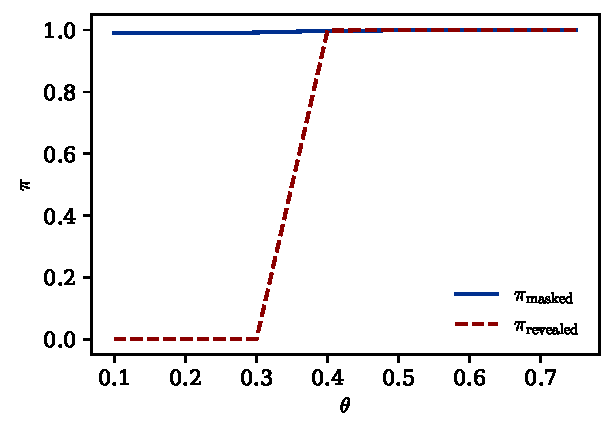
\includegraphics[width=0.62\textwidth]{figures/fig-adv.pdf}
\caption{Masked versus revealed clearing probability across market difficulty $\theta$,
at the reference calibration. The revealed game collapses exactly ($\pir=0$) in the
contested regime; masked momentum is sustained throughout. The masking advantage at
$\theta\le0.30$ is $+0.99$.}
\label{fig:adv}
\end{figure}

% ------------------------------------------------------------------
% P2-statement.tex --- Proposition \ref{prop:selection} ($\lambda$-free
% selection: masked momentum and the contested-regime masking
% advantage) and the diagonal-ignition conjecture
% (Conjecture \ref{conj:DI}). Statement only; the full setup and proof
% are in appendix/P2-proof.tex. Converted from
% docs/propositions-workdir/P2-draft.md (frozen content). Notation:
% the draft's V_1 is written V; \pi_{\mathrm{m}} and \pi_{\mathrm{r}}
% abbreviate the draft's \pi_{masked} and \pi_{rev}.
% ------------------------------------------------------------------

\noindent\textbf{Notation.} At support count $m$ write $g(m) := K - m$ (gap) and $n(m) := N - m$ (uncommitted agents). $A[m,h] \in \{0,1\}$ is the action selected by the masked ($\lambda$-free CvD/Laplacian) rule at state $(m,h)$; $\pi_{\mathrm{m}}$ and $\pi_{\mathrm{r}}$ are the clearing probabilities $P_c[0,T]$ of the masked and revealed games, and $\mathrm{Adv} := \pi_{\mathrm{m}} - \pi_{\mathrm{r}}$. $q_j(n) := \int_0^1 \operatorname{Binom}(n-1,\, p\alpha)(j)\, d\alpha$ is the Laplacian co-mover law. \emph{DI (diagonal ignition)} is the property that the masked rule selects commit at every diagonal state: $A[K-g,\, g] = 1$ for $g = 1, \dots, K$. The momentum bound is $\widehat P(\gamma) := \prod_{i=1}^{\gamma} \bigl( 1 - (1-p)^{N-K+i} \bigr)$, with $\widehat P(0) := 1$.

\medskip
\noindent\textbf{Assumptions.}
\begin{itemize}
\item \textbf{(A1) (primitives).} $N \ge 2$, $2 \le K \le N$, $T \ge K$, $p \in (0,1)$, $V > \kappa > 0$, $L_p \ge 0$, $\rho \ge 0$, $\xi \in [0,1]$.
\item \textbf{(A2) (kernel).} The dynamic game and profile-consistent arrays of the setup (appendix, \S 0.1).
\item \textbf{(A3) (masked rule).} The exact-integral CvD/Laplacian stage selection (appendix, \S 0.2). At diagonal volunteer's-dilemma states,
  where strategic complementarities fail, the Laplacian action is adopted as the
  \emph{definition} of stagewise risk dominance, not invoked as an FMP \S6.4 theorem
  (see the appendix scoping remark).
\item \textbf{(A4) (revealed rule).} The pivotality-blend reduced form (appendix, \S 0.3).
\item \textbf{(A5) (free-riding pays).} $\xi V > V - \kappa$, i.e.\ $\xi > 1 - \kappa/V$.
\item \textbf{(A6) (contested regime).} $K - 1 \ge \max(1,\, pN)$.
\item \textbf{(A7) (deadline ignition).} $\xi V \cdot \bigl(1 - q_0(N-K+1)\bigr) < V - \kappa$, where $q_0(n) := \bigl(1 - (1-p)^n\bigr)/(np)$.
\item \textbf{(A8) (rung-2 ignition, used only for the $K = 2$ part).} With $q_j := q_j(N)$ and $\widehat P(1) := 1 - (1-p)^{N-1}$:
  \begin{itemize}
  \item[\textbf{(C2)}] $q_0 \cdot \bigl[\, (V-\kappa+L_p)\cdot \widehat P(1) - L_p + \rho \,\bigr] + q_1 \cdot \rho \;>\; \bigl(\xi V - (V-\kappa)\bigr)\cdot(1 - q_0 - q_1)$;
  \item[\textbf{(C3)}] $L_p \cdot q_0 + \xi V \cdot (1 - q_0 - q_1) \;\ge\; (V-\kappa)\cdot(1 - q_0)$.
  \end{itemize}
\end{itemize}
A5--A6 are the \textbf{contested-regime} hypotheses (the $\theta$-threshold of part (iv)); A7 is the \textbf{momentum-ignition} hypothesis (the $\theta$-threshold of part (ii)). With the v9 grid map $K(\theta) = \lceil (1-\theta)\cdot N \rceil$, A6 reads: $\theta$ lies below the threshold at which the initial gap exceeds the expected per-period mover count (at the v9 calibration, where $pN = 6$ is an integer: $\theta < 1 - p = 0.4$, i.e.\ exactly $\theta \in \{0.10, 0.20, 0.30\}$ on the grid).

\begin{proposition}[$\lambda$-free selection: masked momentum and the contested-regime advantage]\label{prop:selection}
Under A1--A3 the masked game and under A1, A2, A4 the revealed game are well-defined, and no rationality parameter appears anywhere; for fixed primitives $\mathrm{Adv}$ is a single number (no $\lambda$-inversion is possible). Moreover:
\begin{itemize}
\item[(i)] \textup{(Momentum, conditional form.)} If DI holds, then $\pi_{\mathrm{m}} \ge \widehat P(K) > 0$.
\item[(ii)] \textup{(Ignition at the last rung; $\theta$-threshold.)} Under A7, the masked rule commits at the deadline-pivotal diagonal state: $A[K-1,\, 1] = 1$. Since $q_0(n)$ is strictly decreasing in $n$, A7 is downward-closed in $\theta$: if it holds at threshold $K$ it holds at every $K' \ge K$, i.e.\ for every harder (lower-$\theta$) market.
\item[(iii)] \textup{(Momentum, unconditional for $K = 2$.)} Let $K = 2$ and assume A5, A7, A8. Then DI holds --- $A[1,1] = 1$ and $A[0,2] = 1$ --- and therefore
\[
\pi_{\mathrm{m}} \;\ge\; \widehat P(2) \;=\; \bigl(1 - (1-p)^{N-1}\bigr)\bigl(1 - (1-p)^N\bigr) \;>\; 0.
\]
The hypothesis set is non-vacuous: $(N,K,T,p) = (10, 2, 10, 1/10)$ with the v9 payoffs $(V, \kappa, L_p, \rho, \xi) = (3, 1, 3, 1/20, 4/5)$ satisfies A1, A5, A6, A7, A8 simultaneously (exact margins in the appendix proof, Step 5).
\item[(iv)] \textup{(Revealed collapse in the contested regime.)} Under A1, A2, A4, A5, A6: $\pi_{\mathrm{r}} = 0$ exactly. In particular at the v9 calibration $(N, p) = (10, 3/5)$, A6 holds iff $K \ge 7$, i.e.\ iff $\theta \in \{0.10, 0.20, 0.30\}$ on the v9 grid.
\item[(v)] \textup{(Masking advantage.)} Under the hypotheses of (iv) together with DI (or, for $K = 2$, with A7--A8 instead of DI): $\mathrm{Adv} = \pi_{\mathrm{m}} \ge \widehat P(K) > 0$ --- strictly positive on the contested regime. Globally (without A5--A6), under DI: $\mathrm{Adv} \ge \widehat P(K) - 1$. (No claim of $\mathrm{Adv} \ge 0$ outside the contested regime is made: the ground-truth computation exhibits $\mathrm{Adv} \in [-8 \cdot 10^{-4},\, 0)$ on the easy regime; see Remark R4 in the appendix.)
\end{itemize}
\end{proposition}

\begin{conjecture}[Diagonal ignition at the v9 calibration]\label{conj:DI}
At $(N,T,p,V,\kappa,L_p,\rho,\xi) = (10, 10, 3/5, 3, 1, 3, 1/20, 4/5)$ and every $K \in \{3, \dots, 9\}$ of the v9 $\theta$-grid, DI holds at \emph{every} diagonal rung (and, additionally, the masked rule waits at every below-diagonal state). This is verified pointwise by the ground-truth solver at all seven grid points; parts (i) and (v) of Proposition~\ref{prop:selection} then apply at the calibration. What would close it: a proof of the diagonal stage inequality at rungs $g \ge 2$, which requires an upper bound on the on-cone uncommitted value $V_u$ strictly below $\xi V$ by a margin of order $\xi V \cdot (1 - P_c) + \rho$; the crude bound $V_u \le \xi V$ used in the present technique yields a sufficient condition that is strictly negative at the calibration, while the true (verified) deepest-rung stage margin is $+0.417$. See Remark R3 in the appendix.
\end{conjecture}


The contested-regime collapse --- part (iv) --- is exact and fully proven: when
free-riding pays ($\xi > 1-\kappa/V$) and the market is contested, the pivotality weight
classifies every mover as inframarginal, revelation triggers the free-ride action, and
$\pir = 0$ identically. The momentum floor is proven conditional on diagonal ignition
(property DI), which is itself proven outright at the deadline rung and unconditionally
for $K=2$; at interior rungs for $K\ge3$ it is Conjecture~\ref{conj:DI}, verified
pointwise at every calibration grid point. The precise reading of the advantage: strictly
positive when contested, near-tie elsewhere (the numerics give $-8\times10^{-4}$ at
$\theta=0.40$ --- ``$\ge 0$ everywhere'' is false and we do not claim it).

\subsection{The bundled dial}

Why is the optimal masking \emph{partial}? With both channels live in the dynamic game on
the single bundled dial, a genuine interior optimum exists (Figure~\ref{fig:Gk}).

\begin{figure}[t]
\centering
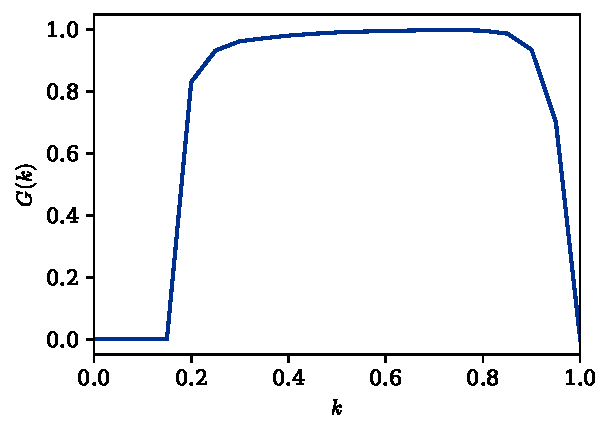
\includegraphics[width=0.62\textwidth]{figures/fig-Gk.pdf}
\caption{The bundled-dial inverted-U\@. Activation gain $G(k)$ at the reference contested
calibration ($\theta=0.30$, $\xi=0.667$, $T=10$): both endpoints are dead --- full masking
cannot ignite momentum, full disclosure fully unravels --- and the interior peak near
$k=0.70$ carries the entire welfare range.}
\label{fig:Gk}
\end{figure}

% ------------------------------------------------------------------
% P3 statement (main-text include): compact assumptions, Proposition
% \ref{prop:bundle} parts (i)-(iii), Conjecture \ref{conj:interiorT},
% Observation \ref{obs:leakagehelps}, Conjecture \ref{conj:decoupledT},
% and the one-sentence falsification pointer. No proofs here; full
% setup, lemmas, proofs, and the falsification record are in
% appendix/P3-proof.tex.
%
% NOTE: this file and P3-proof.tex both carry \label{prop:bundle} and
% the conjecture/observation labels -- include exactly one of the two
% labeled statements in a given document (or strip labels from one).
% Requires amsthm environments: proposition, assumption, conjecture,
% observation.
% ------------------------------------------------------------------

\begin{assumption}\label{ass:bundle}
In the activation game $\Gamma_T(k_{\mathrm{type}},k_{\mathrm{piv}})$ (setup M1--M6 in the
appendix; bundled dial $k_{\mathrm{type}}=k_{\mathrm{piv}}=k$):
\textup{(A0)} regularity: $N\ge 2$; $K\in\{2,\dots,N\}$; $p_{\mathrm{opp}}\in(0,1)$;
$0<\kappa<V$; $L>0$; $L_p>0$; $\rho\ge 0$; $\pi_b\in(0,1)$; $\xi\in(0,1]$.
\textup{(A1)} pessimistic pooling: $0\le\mathbb E<\kappa$, where
$\mathbb E:=(1-\pi_b)V-\pi_b L$.
\textup{(A2)} free-ride regime: $\varepsilon:=\xi V-(V-\kappa)>0$, i.e.\ $\xi>1-\kappa/V$, so
the gate $\chi=1$.
\textup{(A3)} thin root field: $K-1\ge p_{\mathrm{opp}}N$, so $\mathrm{piv}(0)=0$.
\textup{(A4)} pivotal ignition at full type-news: with $X\sim\mathrm{Binom}(N-1,
p_{\mathrm{opp}})$ and $\beta_1=\Pr(X=K-1)$, $\beta_+=\Pr(X\ge K)$, $\beta_-=\Pr(X\le K-2)$:
$(V-\kappa)\,\beta_1>\varepsilon\,\beta_++L_p\,\beta_-$.
\textup{(A5)} small waiting friction: $\rho\,(T-1)<\min\{L_p,\;\kappa-\mathbb E\}$ (vacuous at
$T=1$).
\end{assumption}

\begin{proposition}[bundled-dial interior optimum; decoupled-dial corner]\label{prop:bundle}
\leavevmode
\begin{itemize}
\item[(i)] \textbf{Bundled dial: both corners dead, a live interior, every optimum interior.}
\emph{Endpoints (any horizon).} Under A0, A1, A2, A3, A5, for every $T\ge 1$, the bundled game
satisfies
\[
G(0)=0,\ \ s(0)=1,\qquad G(1)=0,\ \ s(1)=1,\quad\text{hence}\quad W(0)=W(1)=0 .
\]
($k=0$: pooled news cannot ignite momentum --- the unique stage equilibrium is $q=0$ at every
state; $k=1$: full pivotality leakage makes the empty state absorbing --- every root-state mover
free-rides.)
\emph{Interior (one round).} If in addition A4 holds and $T=1$, there is a threshold
$\bar k\in(0,1)$ --- the unique root of the affine root-state differential $D_1$ of the
appendix ignition lemma --- such that for every $k\in[\bar k,1)$:
\begin{gather*}
G(k)=\Pr\!\big(\mathrm{Binom}(N,\;p_{\mathrm{opp}}(1-k))\ge K\big)>0,\qquad s(k)=1,\\
W(k)=(1-\pi_b)\,V\,G(k)>0 .
\end{gather*}
Moreover $W:[0,1]\to\mathbb R$ is upper semicontinuous, attains its maximum, and \textbf{every
maximizer lies in the open interval $(0,1)$}.
\item[(ii)] \textbf{Decoupled dials: the optimum is the corner.} Under A0--A5 and $T=1$, the
decoupled welfare satisfies, for all $(k_{\mathrm{type}},k_{\mathrm{piv}})\in[0,1]^2$,
\[
W(k_{\mathrm{type}},k_{\mathrm{piv}})\;\le\;W(1,0)\;=\;(1-\pi_b)\,V\,
\Pr\!\big(\mathrm{Binom}(N,p_{\mathrm{opp}})\ge K\big)\;>\;0,
\]
and the argmax set is \textbf{exactly} $[\bar k,1]\times\{0\}$ (with $\bar k$ from part (i)):
every optimum has \emph{zero} pivotality leakage and \emph{full ignition}, and
$(k_{\mathrm{type}},k_{\mathrm{piv}})=(1,0)$ attains the optimum. In particular every point
with $k_{\mathrm{piv}}>0$ is strictly suboptimal.
\item[(iii)] \textbf{The interior is a constrained optimum created by bundling.} Under A0--A5
and $T=1$: $\sup_{k\in[0,1]}W(k,k)\le W(1,0)$, and the bundled diagonal never attains $W(1,0)$
(every diagonal point has $a_{\mathrm{eff}}<1$). The bundled optimum is interior (part (i))
while the unconstrained two-dial optimum is the corner (part (ii)); the interior $k^*$ is the
constrained optimum of one dial forced to move both channels together --- not a
type-versus-pivotality balance.
\end{itemize}
\end{proposition}

\begin{conjecture}[general-horizon interior]\label{conj:interiorT}
Under A0--A3, A5, and a strengthened ignition condition, for every $T\ge 1$ there exists
$k\in(0,1)$ with $G(k)>0$ in the bundled game. (Proved at $T=1$; open for $T\ge 2$.)
\end{conjecture}

\begin{observation}[positive leakage can strictly help at $T\ge 2$]\label{obs:leakagehelps}
There exist instances satisfying A0--A5, horizons $T\ge 2$, and dials
$k_{\mathrm{type}}\in[0,1]$, $k_{\mathrm{piv}}>0$ such that
$W(k_{\mathrm{type}},k_{\mathrm{piv}})>W(k_{\mathrm{type}},0)$ with $s\equiv 1$ at both
points: positive pivotality leakage is strictly welfare-improving, through the good-coalition
continuation/waiting-option channel. At $T=1$ this is impossible
(Proposition~\ref{prop:bundle}(ii)), so the phenomenon is strictly dynamic. (Verified
instance in the appendix.)
\end{observation}

\begin{conjecture}[narrowed residual conjecture: decoupled argmax retains $k_{\mathrm{piv}}=0$]\label{conj:decoupledT}
Under A0--A5, for every $T\ge 1$ the decoupled welfare attains its maximum at some point with
$k_{\mathrm{piv}}=0$ --- with no claim that $(1,0)$ attains it, and no pointwise dominance
claim in $k_{\mathrm{piv}}$. (Theorem at $T=1$ by Proposition~\ref{prop:bundle}(ii); open for
$T\ge 2$.)
\end{conjecture}

The original general-horizon decoupled-corner conjecture --- that under A0--A5 the decoupled
argmax has $k_{\mathrm{piv}}=0$ and is attained at $(1,0)$ for every $T\ge 1$ --- was falsified
in verification by an explicit A0--A5 counterexample at $T\in\{2,5,10\}$; the falsification
record, counterexample parameters, and replication notes appear in the appendix
(Remark~\ref{rem:falsifiedC2}).


The decoupled-dial result --- part (iii) --- is what makes the interior structural rather
than incidental: with two separate dials, the optimum is the corner
$(\ktype,\kpiv)=(1,0)$, full type-disclosure with zero pivotality leakage. The bundled
interior is therefore a \emph{constrained} optimum created by the yoking --- one physical
dial cannot certify a coalition's reality without leaking its pivotal structure --- and
never a type-versus-pivotality balance. Partial masking thus has two distinct sources:
the integrity-distribution shape (Proposition~\ref{prop:band}) and the one-dial coupling
(Proposition~\ref{prop:bundle}).

Horizon scope: parts (ii)--(iii) are $T=1$ theorems; the endpoint results hold at
every horizon. At $T\ge2$ the original general-horizon decoupled-corner conjecture was
\emph{falsified} in adversarial verification --- within the proposition's own assumptions,
the corner can fail to be attained, and positive pivotality leakage can strictly improve
welfare at fixed type-disclosure (Observation~\ref{obs:leakagehelps}): a leakier future
cuts the waiting option and re-ignites mid-states through the continuation channel.
Whether the decoupled argmax always retains $\kpiv=0$ is open
(Conjecture~\ref{conj:decoupledT}). The leakage-helps phenomenon is itself a new,
empirically probeable prediction.

% =====================================================================
\section{Boundary: where the theorem reverses}\label{sec:boundary}

The theorem is conditional on the walls actually being down.

\emph{$q$ collapses.} Authentication is weak; masked disclosure now shields
\emph{manufactured} commitments rather than protecting a real coalition. ``Minimal
disclosure'' flips from efficient to fraud-enabling. Below the located threshold
(the joint region requires $q\gtrsim0.95$), transparency dominates.

\emph{$c$ collapses.} The conditional structure is illusory --- nodes are real but their
conditions are not jointly satisfiable; clearing produces no activatable outcome. The
masking band is interior in $c$ (Proposition~\ref{prop:band}): below it, screening
dominates and transparency wins; above it, coalitions are too robust to unravel and
disclosure is harmless.

\emph{The contested regime is absent.} The protection channel matters only where the
static selection frontier binds and free-riding pays ($\xi > 1-\kappa/V$): a good
coalition that exists but would unravel if its pivotal structure were exposed. Where
completion is easy, masking is neutral (the near-tie region of
Proposition~\ref{prop:selection}).

\emph{Endogeneity over-extends.} If outcome terms stay fuzzy past the binding moment, the
campaign instrument is indeterminate; precision must harden as commitment strength rises
(the interior $\sigma^*$ under high indeterminacy cost).

\emph{The taxonomy over-expands.} ``Interdependent action'' becomes a slogan unless every
example reduces to a conditional-commitment graph --- nodes, edges, constraints, fixed
point. The family is broad; the primitive must stay narrow.

% =====================================================================
\section{Mechanism and an administrable rule}\label{sec:rule}

\paragraph{Mechanism.} A no-custody clearinghouse for conditional commitments with
(a)~authenticated nodes, (b)~verifiable conditional structure, (c)~endogenous outcome
terms with a hardening schedule, (d)~partial disclosure (an interior $k$-anonymity level)
on granular state, (e)~value riding the recipient's own rail, and (f)~non-transferable
participant commitments.

\paragraph{Normative rule.} We propose model-motivated design criteria for a limited
safe harbor for a privacy-preserving conditional-commitment clearinghouse --- a proposed
administrable rule, not a legal conclusion, and pending counsel review. The four criteria:
non-transferable participant commitments; no custody of principal; an auditable
node-authentication process; and small-$N$ disclosure controls. The rule regulates the
\emph{clearing of commitments} --- not raw wishes, raw data, platform funds, or
transferable financial instruments --- and is keyed to the conditional-commitment
structure, not the campaign's vertical. The theory motivates each prong: the
authentication prong is the $q$-collapse boundary; the disclosure-controls prong is the
small-$N$ regime where the dynamic protection effect (and its abuse surface) lives; the
no-custody and non-transferability prongs keep the cleared object a coordination device
rather than a financial instrument.

% =====================================================================
\section{Implementation: a constructive implementability case}\label{sec:constructive}

The empirical spine is not yet a dataset --- it is a live platform's release history,
readable as a constructive case that the institution is implementable. Implementability is
all this section claims: a release history cannot validate optimality, welfare, or the
selection results, and the calibration quantities are unmeasured
(Section~\ref{sec:empirics}). The
platform (ifwishlist, live June 2026) did not ship unrelated features; it removed the four
walls one at a time: authenticated counterpart resolution (credibility, $q$); a
conditional-commitment grammar with compound and roster thresholds (compatibility, $c$);
semantic routing (discoverability); a no-custody rail (legality); and the $k$-anonymity
dial with a specification-hardening schedule --- an architecture consistent with the
model's recommended design.

% =====================================================================
\section{Empirical agenda}\label{sec:empirics}

The theory chain has largely converged; the marginal value has moved to measurement. Four
quantities, all currently unmeasured, each first-order for a specific result:

\begin{center}
\begin{tabular}{lll}
\toprule
\textbf{Quantity} & \textbf{Governs} & \textbf{Disciplines} \\
\midrule
support gap $p_G - p_B$ & the screening cap $s(1)$, large-gap reversal & \S\ref{sec:dial} \\
excludability $\xi$ & which channel regime governs & \S\ref{sec:dial}--\ref{sec:selection} \\
campaign-size distribution & the scale of the finite-$N$ protection effect & \S\ref{sec:central} \\
$\pi_b$ and the integrity distribution & band location; interior $k^*$ & Prop.~\ref{prop:band}, \ref{prop:bundle} \\
\bottomrule
\end{tabular}
\end{center}

A further theory iteration is warranted only when a measured quantity makes a specific
model question first-order. Observation~\ref{obs:leakagehelps} adds a sharp new item:
the leakage-helps regime is directly probeable on live activation data.

% =====================================================================
\section{Scope, open questions, and the verification record}\label{sec:scope}

Every numerical claim in this paper comes from a chain of solver scripts under fixed
seeds, and every analytical result was drafted against those scripts as ground truth and
then attacked by three separately instantiated adversarial verification passes --- a
step-by-step logic audit, a counterexample hunt running randomized parameter sweeps inside
the stated assumption sets, and a scope audit of claim--proposition alignment --- each run
with no access to the others' findings, with scripts and logs archived alongside the
numerical companion. Roughly
$3{,}500$ randomized counterexample instances were run against the stated assumption sets;
no proved statement was refuted. The process corrected the first draft of every artifact
it touched --- including four sections of this paper --- and falsified one of our own
conjectures, producing Observation~\ref{obs:leakagehelps}. We report the open residue explicitly:

\begin{enumerate}
\item \textbf{Conjecture~\ref{conj:connected}} (connectedness of the masking band): the
lower transition is a discontinuous global-max switch with no first-order
characterization.
\item \textbf{Conjecture~\ref{conj:DI}} (diagonal ignition at interior rungs): closing it
needs a simultaneous induction bounding the on-cone waiting value.
\item \textbf{Conjecture~\ref{conj:interiorT}} (the $T>1$ interior): numerically robust;
the band grows with horizon.
\item \textbf{Conjecture~\ref{conj:decoupledT}} (decoupled argmax retains zero leakage):
open after refinement; the pointwise version is false
(Observation~\ref{obs:leakagehelps}).
\item Deriving $(p_G,p_B)$ from a deeper compatibility primitive; correlated signals; an
endogenous adverse-selection prior $\pi_b$.
\end{enumerate}

Two further scope notes. The legality-wall claim inherits open predicates pending counsel
review (the no-custody rail's money-transmission posture; charitable-solicitation
regimes). And the live system does not yet instrument $q$ or $c$; both are required for
the central theorem to bite on data.

% =====================================================================
\section{Conclusion}\label{sec:conclusion}

AI does not make the engine intelligent. It removes two of the four walls --- credibility
and discoverability --- that kept interdependent willingness from ever clearing. The
mechanism removes the third (compatibility); the legal architecture removes the fourth.
With all four down, ``I would, if\ldots'' becomes a clearable economic object --- and the
efficient clearinghouse is the one that holds nothing, fixes nothing early, and hides the
granular.

\bibliographystyle{plainnat}
\bibliography{references}

\clearpage
\appendix

\section{Proof of Proposition~\ref{prop:band}}\label{app:P1}
% ---------------------------------------------------------------------------
% P1-proof.tex --- appendix: setup, lemmas, proof, and remarks for
% Proposition \ref{prop:band} (interior masking band in consensus integrity).
% Statement lives in appendix/P1-statement.tex (included in the paper body).
% Converted from docs/propositions-workdir/P1-draft.md (content frozen;
% notation renames only: kappa -> eta, theta -> r per the paper's canon).
% Two bound-variable renames forced by the notation map, with no change in
% content: the draft's local eta in the masking lemma is written delta here
% (eta now denotes the Beta concentration), and the draft's ratio r(c) in the
% upper-threshold lemma is written lambda(c) (r now denotes robustness).
% ---------------------------------------------------------------------------

{\sloppy
\noindent\emph{Provenance.} This appendix formalizes the v2 $c$-axis reversal / v3
``$k^*$-valley'' claim. Ground truth for the model is
\texttt{docs/lit/conditional-commitment/}\allowbreak\texttt{runs/numcheck/v3.py} and
\texttt{v3\_shape.py}; the headline anchor sequence is produced by
\texttt{v7\_unify.py}~\S0 (see Remarks~\ref{rem:anchors} and~\ref{rem:q1} for its exact
parameters). The proof below stands without them.\par}

\subsection*{Setup and assumptions}

\paragraph{Model (restricted variant of toy model v3, matching the scripts exactly).}
A platform chooses a disclosure granularity $k \in [0,1]$ ($k = 1$ full disclosure,
$k = 0$ full masking). A coalition is \emph{good} with probability $qc$ and \emph{bad}
with probability $1 - qc$, where $q \in (0,1]$ is authentication accuracy and
$c \in (0,1)$ is consensus integrity. A good coalition has robustness $r_g \sim F_c$ on
$[0,1]$ and delivers surplus $V > 0$ unless it unravels; unraveling occurs iff
$r_g < \hat r(k)$, where $\hat r(k)$ is the strategic activation cutoff induced by
disclosure level $k$, so the unraveling risk is $\rho(k,c) = F_c(\hat r(k))$. A bad
coalition imposes loss $L > 0$ unless screened, which happens with probability $s(k)$.

\paragraph{Restriction (linear channels).} Throughout we take the channels in the exact
form used by the numerical scripts:
\[
\hat r(k) = \tau k \quad \text{with } \tau \in (0,1)
\quad \text{(v2 Lemma~1 transparency cutoff at $k = 1$)},
\qquad
s(k) = k.
\]
(Toy model v3 allows general $C^1$ increasing channels with these endpoints; we prove
the result for the linear specification only. See Remark~\ref{rem:restriction}.)

Welfare:
\begin{equation}
W(k; q, c) \;=\; qcV\bigl(1 - F_c(\tau k)\bigr) \;-\; (1 - qc)\,L\,(1 - k).
\tag{W}\label{eq:W-app}
\end{equation}
Let $K^*(c) := \operatorname*{arg\,max}_{k \in [0,1]} W(k; q, c)$ (the dependence on
$q$ is suppressed except in part~(e)). We write ``full disclosure is uniquely optimal
at $c$'' for $K^*(c) = \{1\}$ and ``masking is optimal at $c$'' for $1 \notin K^*(c)$.
Define the \emph{masking set}
\[
M \;:=\; \{\, c \in (0,1) : 1 \notin K^*(c) \,\},
\]
and the \emph{marginal-balance function} (minus the right-hand slope of $W$ at $k = 1$)
\begin{equation}
\varphi(c) \;:=\; qcV\tau f_c(\tau) \;-\; (1 - qc)\,L.
\tag{$\varphi$}\label{eq:phi-app}
\end{equation}
$\varphi(c) > 0$ says: at full disclosure, the marginal unraveling loss
$qcV\tau f_c(\tau)$ exceeds the marginal screening gain $(1 - qc)L$.

\paragraph{Assumptions.}
\begin{assumptionlist}
\item[\textbf{(A1) (payoffs).}] $V, L > 0$, $\tau \in (0,1)$, $q \in (0,1]$,
  $c \in (0,1)$; welfare is \eqref{eq:W-app}.
\item[\textbf{(A2) (linear channels --- restriction).}] $\hat r(k) = \tau k$,
  $s(k) = k$, hence $\rho(k,c) = F_c(\tau k)$. This is exactly the specification of
  \texttt{v3.py}~/ \texttt{v3\_shape.py}.
\item[\textbf{(A3) (family regularity).}] For each $c \in (0,1)$, $F_c$ is a CDF on
  $[0,1]$ with density $f_c$ strictly positive and continuous on $(0,1)$, and
  $(r, c) \mapsto f_c(r)$ is continuous on $(0,1) \times (0,1)$.
\item[\textbf{(A4) (fragile-end thinness at the cutoff).}] There exists
  $\bar k \in (0,1)$ with
  \[
  \lim_{c \to 0^+} \; c \, \sup_{r \in [\tau\bar k,\, \tau]} f_c(r) \;=\; 0.
  \]
  (At very low integrity, the robustness density of good coalitions carries vanishing
  $c$-weighted mass near the transparency cutoff $\tau$.)
\item[\textbf{(A5) (robust-end thinness below the cutoff).}]
  {\sloppy
  $\lim_{c \to 1^-} S(c) = 0$, where $S(c) := \sup_{r \in (0,\tau]} f_c(r)$, and
  \textbf{either} (i) $q < 1$, \textbf{or} (ii)
  \[
  \limsup_{c \to 1^-} \; \frac{cV\tau S(c)}{(1 - c)L} \;<\; 1.
  \]
  (At very high integrity, good coalitions are too robust to unravel: the density on
  $[0, \tau]$ vanishes --- fast enough, relative to $1 - c$, if $q = 1$.)\par}
\item[\textbf{(A6) (interior bite --- non-vacuity).}] There exists $c_m \in (0,1)$ with
  $\varphi(c_m) > 0$, i.e.
  \[
  q\, c_m V \tau f_{c_m}(\tau) \;>\; (1 - q c_m)\, L.
  \]
\item[\textbf{(A7) (Beta specialization, for parts (d)).}]
  $F_c = \mathrm{Beta}\bigl(c\eta, (1-c)\eta\bigr)$ on $[0,1]$ with fixed concentration
  $\eta > 2$ (mean $c$; the family of v2/v3 and of \texttt{v3\_shape.py}). Define
  \[
  \bar c \;:=\; \frac{1 + \tau(\eta - 2)}{\eta} \;\in\; \Bigl(\frac{1}{\eta},\, 1\Bigr)
  \qquad \text{(the concavity threshold)},
  \]
  the smallest $c$ at which the Beta mode $(c\eta - 1)/(\eta - 2)$ reaches $\tau$.
\end{assumptionlist}

Note: \textbf{first-order stochastic dominance of $\{F_c\}$ in $c$ is nowhere used};
what drives the band is the behavior of the density at and below the cutoff $\tau$ (A4,
A5, A6). FOSD with fixed support is the natural way such behavior arises
(Remark~\ref{rem:fosd}). Lemma~\ref{lem:beta-family} below proves that the Beta family
satisfies A3, A4, and the first part of A5.

\subsection*{Proof of Proposition~\ref{prop:band}}

Throughout fix $q \in (0,1]$ and suppress it except where varied. From
\eqref{eq:W-app}, since $F_c$ is continuous (A3 gives a density), $W(\cdot\,; c)$ is
continuous on the compact $[0,1]$; $K^*(c) \neq \emptyset$. This proves
part~\textbf{(a)}. For $k \in (0,1]$, $W(\cdot\,; c)$ is differentiable with
\begin{equation}
W'(k; c) \;=\; (1 - qc)\,L \;-\; qcV\tau f_c(\tau k),
\tag{D}\label{eq:D}
\end{equation}
continuous in $k$ on $(0,1]$ (one-sided at $k = 1$) because $f_c$ is continuous on
$(0,1)$ and $0 < \tau k \le \tau < 1$. Since $F_c$ is $C^1$ on $(0,1)$,
$W(\cdot\,; c)$ is absolutely continuous on $[0,1]$ and for $0 \le k \le 1$,
\begin{equation}
W(1; c) - W(k; c) \;=\; (1 - qc)\,L\,(1 - k) \;-\; qcV\bigl[F_c(\tau) - F_c(\tau k)\bigr].
\tag{$\star$}\label{eq:star}
\end{equation}
(\eqref{eq:star} is also immediate by direct substitution into \eqref{eq:W-app}.) Note
$W'(1; c) = -\varphi(c)$.

\begin{lemma}[Low integrity: full disclosure uniquely optimal]\label{lem:low}
Under A1--A4 there exists $c_1 > 0$ such that for all $c \in (0, c_1)$:
$W(1; c) > W(k; c)$ for every $k \in [0,1)$, i.e.\ $K^*(c) = \{1\}$.
\end{lemma}

\begin{proof}
Let $\bar k$ be as in A4 and write
$\varepsilon(c) := c \, \sup_{r \in [\tau\bar k,\, \tau]} f_c(r) \to 0$ (A4).

\emph{Case $k \in [\bar k, 1)$.} Then $\tau k \ge \tau\bar k$, so
\[
F_c(\tau) - F_c(\tau k)
= \int_{\tau k}^{\tau} f_c(r)\, dr
\le \tau (1 - k) \sup_{r \in [\tau\bar k,\, \tau]} f_c(r),
\]
using that the integrand is bounded by the sup over
$[\tau\bar k, \tau] \supseteq [\tau k, \tau]$ and the interval has length
$\tau(1 - k)$. Substituting into \eqref{eq:star}:
\[
W(1; c) - W(k; c) \;\ge\; (1 - k)\bigl[\, (1 - qc)\,L - qV\tau\,\varepsilon(c) \,\bigr].
\]
Since $qc \le q \le 1$ and $c \to 0$, $(1 - qc)L \to L > 0$ while
$qV\tau\,\varepsilon(c) \to 0$; choose $c_1' > 0$ such that for $c < c_1'$ the bracket
is strictly positive. Then $W(1) > W(k)$ for all $k \in [\bar k, 1)$.

\emph{Case $k \in [0, \bar k]$.} Bound $F_c(\tau) - F_c(\tau k) \le 1$ in
\eqref{eq:star}:
\[
W(1; c) - W(k; c) \;\ge\; (1 - qc)\,L\,(1 - \bar k) - qcV,
\]
which is strictly positive once $qcV < (1 - qc)\,L\,(1 - \bar k)$; since the left side
$\to 0$ and the right side $\to L(1 - \bar k) > 0$ as $c \to 0$, there is $c_1'' > 0$
below which it holds.

Take $c_1 := \min(c_1', c_1'')$.
\end{proof}

\begin{lemma}[High integrity: full disclosure uniquely optimal]\label{lem:high}
Under A1--A3 and A5 there exists $c_2 < 1$ such that for all $c \in (c_2, 1)$:
$W'(k; c) > 0$ for every $k \in (0,1]$, hence $W(\cdot\,; c)$ is strictly increasing on
$[0,1]$ and $K^*(c) = \{1\}$.
\end{lemma}

\begin{proof}
From \eqref{eq:D}, for every $k \in (0,1]$,
$W'(k; c) \ge (1 - qc)L - qcV\tau S(c)$ with $S(c) = \sup_{(0,\tau]} f_c$.

\emph{Case A5(i) ($q < 1$).} $(1 - qc)L \ge (1 - q)L > 0$ for all $c$, while
$qcV\tau S(c) \le V\tau S(c) \to 0$ as $c \to 1$ (A5). So there is $c_2 < 1$ past which
the lower bound is strictly positive.

\emph{Case A5(ii).} $(1 - qc)L \ge (1 - c)L$ (since $q \le 1$). By A5(ii) there are
$\delta > 0$ and $c_2 < 1$ with $cV\tau S(c) \le (1 - \delta)(1 - c)L$ for
$c \in (c_2, 1)$; then
$W'(k; c) \ge (1 - c)L - q(1 - \delta)(1 - c)L \ge \delta(1 - c)L > 0$.

A continuous function with strictly positive derivative on $(0,1]$ is strictly
increasing on $[0,1]$ (absolute continuity, noted above), so the unique maximizer is
$k = 1$.
\end{proof}

\begin{lemma}[Intermediate integrity: masking strictly optimal]\label{lem:mask}
Under A1--A3 and A6: $1 \notin K^*(c_m)$.
\end{lemma}

\begin{proof}
By \eqref{eq:D} and A6, $W'(1; c_m) = -\varphi(c_m) < 0$. $W'(\cdot\,; c_m)$ is
continuous on $(0,1]$, so there is $\delta \in (0,1)$ with $W' < 0$ on
$[1 - \delta, 1]$; integrating,
$W(1 - \delta; c_m) - W(1; c_m) = -\int_{1-\delta}^{1} W' > 0$. Hence $k = 1$ is not a
maximizer.
\end{proof}

\begin{proof}[Proof of parts (b) and (c)]
Part (b) is Lemmas~\ref{lem:low} and~\ref{lem:high}. For (c):
Lemma~\ref{lem:mask} gives $c_m \in M$, so $M \neq \emptyset$ and
$c_{\mathrm{lo}} = \inf M \le c_m \le \sup M = c_{\mathrm{hi}}$. Lemma~\ref{lem:low}
gives $M \cap (0, c_1) = \emptyset$, so $c_{\mathrm{lo}} \ge c_1 > 0$;
Lemma~\ref{lem:high} gives $M \cap (c_2, 1) = \emptyset$, so
$c_{\mathrm{hi}} \le c_2 < 1$. If $c < c_{\mathrm{lo}}$ then $c \notin M$ (by
definition of the infimum no element of $M$ lies below $c_{\mathrm{lo}}$), i.e.\
$1 \in K^*(c)$; symmetrically for $c > c_{\mathrm{hi}}$. Uniqueness on
$(0, c_1) \cup (c_2, 1)$ is the uniqueness in
Lemmas~\ref{lem:low}--\ref{lem:high}.
\end{proof}

\begin{lemma}[The Beta family satisfies A3, A4, and the first part of A5]
\label{lem:beta-family}
Let $F_c = \mathrm{Beta}(a, b)$ with $a = c\eta$, $b = (1 - c)\eta$, $\eta > 2$ (A7).
Then A3 holds; A4 holds for every $\bar k \in (0,1)$, with
$\sup_{[\tau\bar k,\, \tau]} f_c(r) \to 0$ (not merely $c \cdot \sup \to 0$); and
$S(c) = \sup_{(0,\tau]} f_c(r) \to 0$ as $c \to 1^-$. Moreover the A5(ii) ratio has the
explicit limit
\begin{equation}
\limsup_{c \to 1^-} \; \frac{cV\tau S(c)}{(1 - c)L}
\;=\; \frac{\eta V \tau^{\eta}}{(1 - \tau)L}.
\tag{A5$'$}\label{eq:A5prime}
\end{equation}
\end{lemma}

\begin{proof}
Write $f_c(r) = r^{a-1}(1 - r)^{b-1}/B(a, b)$,
$B(a, b) = \Gamma(a)\Gamma(b)/\Gamma(\eta)$ (using $a + b = \eta$). Joint continuity
and positivity on $(0,1)^2$ is standard (continuity of $\Gamma$ on $(0,\infty)$ and of
powers); A3 holds.

\emph{A4.} Fix $\bar k \in (0,1)$ and take $c < \min(1/\eta, 1/2)$, so $a < 1$ and
$b > \eta/2 \ge 1$. For $r \in [\tau\bar k, \tau]$:
$r^{a-1} \le (\tau\bar k)^{a-1} \le (\tau\bar k)^{-1}$ (exponent negative,
$r \ge \tau\bar k$, and $(\tau\bar k)^{a-1} \le (\tau\bar k)^{-1}$ since
$\tau\bar k < 1$ and $a > 0$), and $(1 - r)^{b-1} \le 1$ ($b \ge 1$, $1 - r \le 1$). So
$\sup_{[\tau\bar k,\, \tau]} f_c \le (\tau\bar k)^{-1}/B(a, b)$. Lower-bound $B$: with
$m := \min_{x \in [1,2]} \Gamma(x) > 0$, $\Gamma(a) = \Gamma(a + 1)/a \ge m/a$ for
$a \in (0,1)$; and
$\Gamma(b)/\Gamma(\eta) \ge \gamma_0 := \min_{x \in [\eta/2,\, \eta]}
\Gamma(x)/\Gamma(\eta) > 0$ for $c \le 1/2$. Hence $B(a, b) \ge m\gamma_0/(c\eta)$ and
\[
\sup_{[\tau\bar k,\, \tau]} f_c(r)
\;\le\; \frac{c\eta}{m \gamma_0 \tau \bar k}
\;\to\; 0 \quad \text{as } c \to 0^+.
\]

\emph{A5 first part and \eqref{eq:A5prime}.} Take $c$ close enough to $1$ that $a > 1$
and $b < 1$. On $(0, \tau]$: $(a-1)/r - (b-1)/(1-r) > 0$ (both terms positive), so
$f_c$ is strictly increasing there and $S(c) = f_c(\tau)$. By the same $\Gamma$ bounds
with the roles of $a, b$ swapped, $B(a, b) \ge m\gamma_1/((1 - c)\eta)$ with
$\gamma_1 := \min_{x \in [\eta/2,\, \eta]} \Gamma(x)/\Gamma(\eta) > 0$, so
$S(c) \le (1 - c)\eta\, \tau^{a-1}(1 - \tau)^{b-1}/(m\gamma_1) \to 0$ (the powers stay
bounded: $\tau^{a-1} \le 1$ for $a \ge 1$, $(1 - \tau)^{b-1} \le (1 - \tau)^{-1}$). For
the exact limit: as $c \to 1^-$, $\Gamma(b) \sim 1/b$ ($\Gamma(b) = \Gamma(b + 1)/b$,
$\Gamma(b + 1) \to 1$), $\Gamma(a) \to \Gamma(\eta)$, so
$B(a, b) \sim 1/b = 1/((1 - c)\eta)$ and
\[
S(c) = f_c(\tau) \;\sim\; (1 - c)\,\eta\,\frac{\tau^{\eta - 1}}{1 - \tau},
\]
whence $cV\tau S(c)/((1 - c)L) \to \eta V \tau^{\eta}/((1 - \tau)L)$, which is
\eqref{eq:A5prime}.
\end{proof}

\noindent (Thus under A7 with $q < 1$, A5(i) applies with no further condition; if
$q = 1$, A5(ii) holds iff $\eta V \tau^{\eta} < (1 - \tau)L$. See
Remark~\ref{rem:q1}.)

\begin{lemma}[Beta: strict log-concavity of the marginal-balance ratio --- part (d1)]
\label{lem:logconcave}
Under A7, $g(c) := \log\bigl[\, qcV\tau f_c(\tau) \,/\, ((1 - qc)L) \,\bigr]$ is
strictly concave on $(0,1)$.
\end{lemma}

\begin{proof}
With $a = c\eta$, $b = (1 - c)\eta$:
\[
g(c) = \mathrm{const} + \log c + (c\eta - 1)\log\tau + ((1 - c)\eta - 1)\log(1 - \tau)
- \log B(c\eta, (1 - c)\eta) - \log(1 - qc).
\]
The two power terms are affine in $c$ (second derivative $0$). Using
$\log B(a, b) = \log\Gamma(c\eta) + \log\Gamma((1 - c)\eta) - \log\Gamma(\eta)$ and
$\frac{d^2}{dx^2}\log\Gamma(x) = \psi_1(x)$ (trigamma), the chain rule gives
$\frac{d^2}{dc^2}\log B = \eta^2\psi_1(c\eta) + \eta^2\psi_1((1 - c)\eta)$. Also
$\frac{d^2}{dc^2}\bigl[-\log(1 - qc)\bigr] = q^2/(1 - qc)^2$ and
$\frac{d^2}{dc^2}\log c = -1/c^2$. Hence
\[
g''(c) = -\frac{1}{c^2} - \eta^2\psi_1(c\eta) - \eta^2\psi_1((1 - c)\eta)
+ \frac{q^2}{(1 - qc)^2}.
\]
Two elementary facts close the sign. First,
$\psi_1(x) = \sum_{n \ge 0} (x + n)^{-2} > x^{-2}$ for $x > 0$ (the $n = 0$ term
alone), so $\eta^2\psi_1((1 - c)\eta) > \eta^2/((1 - c)\eta)^2 = 1/(1 - c)^2$. Second,
$1 - qc \ge q(1 - c)$ for $q \le 1$ (equivalent to $1 - q \ge 0$), so
$q^2/(1 - qc)^2 \le q^2/(q^2(1 - c)^2) = 1/(1 - c)^2$. Therefore
\[
g''(c) < -\frac{1}{c^2} - \eta^2\psi_1(c\eta) - \frac{1}{(1 - c)^2}
+ \frac{1}{(1 - c)^2} = -\frac{1}{c^2} - \eta^2\psi_1(c\eta) < 0.
\qedhere
\]
\end{proof}

\noindent Since $\varphi(c) > 0 \iff g(c) > 0$ and $g$ is strictly concave and
continuous, $\{\varphi > 0\}$ is the intersection of $(0,1)$ with an open interval; by
A6 it is nonempty and contains $c_m$. Write it $(c_-, c_+)$. This proves
part~\textbf{(d1)}.

\begin{lemma}[Beta: strict concavity of $W$ in $k$ on the upper shoulder --- part (d2)]
\label{lem:concave}
Under A7, for every $c \in [\bar c, 1)$: $f_c$ is strictly increasing on $(0, \tau)$
with $f_c(0^+) = 0$; consequently $W(\cdot\,; c)$ is strictly concave on $[0,1]$,
$K^*(c) = \{k^*(c)\}$ is a singleton with $k^*(c) > 0$, and
$k^*(c) < 1 \iff \varphi(c) > 0$, in which case $k^*(c)$ solves the FOC
$qcV\tau f_c(\tau k^*) = (1 - qc)L$.
\end{lemma}

\begin{proof}
For $c \ge \bar c$, $a = c\eta \ge 1 + \tau(\eta - 2) > 1$ (definition of $\bar c$;
$\eta > 2$). On $(0,1)$,
\[
\frac{f_c'(r)}{f_c(r)} = \frac{a - 1}{r} - \frac{b - 1}{1 - r}.
\]
If $b \le 1$, both terms are positive on $(0, \tau]$, so $f_c' > 0$ there. If $b > 1$,
$f_c'(r) > 0$ iff $r < m_c := (a - 1)/(a + b - 2) = (c\eta - 1)/(\eta - 2)$, and
$c \ge \bar c \iff m_c \ge \tau$; so $f_c' > 0$ on $(0, \tau)$ (at $r = \tau = m_c$ the
derivative is $0$, harmless). Also $f_c(0^+) = 0$ because $a - 1 > 0$ makes
$r^{a-1} \to 0$ while $(1 - r)^{b-1}/B$ stays bounded near $0$.

By \eqref{eq:D}, $W'(k; c) = (1 - qc)L - qcV\tau f_c(\tau k)$ is then strictly
decreasing in $k$ on $(0,1]$ wherever $\tau k < \tau$ and non-increasing at the
endpoint, with $W'(0^+; c) = (1 - qc)L > 0$. A continuous function on $[0,1]$ whose
derivative exists and is strictly decreasing on $(0,1)$ is strictly concave; its
maximizer is unique. Since $W'(0^+) > 0$, $k^*(c) > 0$. If $\varphi(c) \le 0$, then
$W'(1) = -\varphi(c) \ge 0$ and by strict monotonicity of $W'$, $W'(k) > 0$ for all
$k < 1$: $W$ is strictly increasing, $k^*(c) = 1$. If $\varphi(c) > 0$, then
$W'(1) < 0 < W'(0^+)$, and by continuity and strict monotonicity of $W'$ on $(0,1]$
there is a unique root $k^* \in (0,1)$, the unique maximizer of the strictly concave
$W$; the root condition is exactly the stated FOC.
\end{proof}

\begin{lemma}[Sharp upper threshold and continuity at the upper edge --- part (d3)]
\label{lem:upper}
Under A7, A5(i) or (ii), and A6, suppose $c_+ > \bar c$. Then
$c_{\mathrm{hi}} = c_+ < 1$, $\bigl( \max(\bar c, c_-),\, c_+ \bigr) \subseteq M$, the
maximizer $k^*(\cdot)$ is continuous on $\bigl( \max(\bar c, c_-),\, c_+ \bigr)$, and
$k^*(c) \to 1$ as $c \uparrow c_+$.
\end{lemma}

\begin{proof}
\emph{Location of the threshold.} By Lemma~\ref{lem:high}, for $c \in (c_2, 1)$ we have
$W'(1; c) > 0$, i.e.\ $\varphi(c) < 0$; hence $c_+ \le c_2 < 1$. By
Lemma~\ref{lem:concave}, for $c \in [\bar c, 1)$:
$c \in M \iff \varphi(c) > 0 \iff c \in (c_-, c_+)$ (Lemma~\ref{lem:logconcave}). Since
$c_+ > \bar c$, the set $M \cap [\bar c, 1)$ equals $[\bar c, 1) \cap (c_-, c_+)$,
which contains the nonempty interval $\bigl( \max(\bar c, c_-),\, c_+ \bigr)$; in
particular it contains points arbitrarily close to $c_+$ from below and no point
$\ge c_+$. Any other element of $M$ lies in $(0, \bar c) \subset (0, c_+)$. Hence
$\sup M = c_+$, i.e.\ $c_{\mathrm{hi}} = c_+$.

\emph{Interior solution and continuity.} For
$c \in \bigl( \max(\bar c, c_-),\, c_+ \bigr)$, Lemma~\ref{lem:concave} gives the
unique interior maximizer $k^*(c) \in (0,1)$ solving
$f_c(\tau k^*(c)) = \lambda(c) := (1 - qc)L/(qcV\tau)$. Continuity of $k^*$ on this
interval: if $c_n \to c$ in the interval and (by compactness, along a subsequence)
$k^*(c_n) \to \tilde k \in [0,1]$, two boundary cases are excluded. (i) $\tilde k = 0$
is impossible: for $c$ in a compact neighborhood $[\bar c, c_+] \subset (0,1)$,
$a = c\eta \ge 1 + \alpha$ with $\alpha := \tau(\eta - 2) > 0$, and $B(a, b)$ is
bounded below by a positive constant (continuity and positivity of $B$ on the compact
parameter set), while $(1 - r)^{b-1} \le (1 - \tau)^{b-1}$ is bounded above for
$r \le \tau$; hence $f_c(r) \le C\, r^{\alpha}$ uniformly on that neighborhood, so
$f_{c_n}(\tau k^*(c_n)) \to 0$ if $k^*(c_n) \to 0$, contradicting
$f_{c_n}(\tau k^*(c_n)) = \lambda(c_n) \ge \lambda(c_+) > 0$ ($\lambda$ is strictly
decreasing in $c$, and $1 - qc_+ > 0$ because $c_+ < 1$ and $q \le 1$). (ii) Otherwise
$\tilde k \in (0,1]$ and joint continuity of $f$ (A3, point $(\tau\tilde k, c)$ with
$\tau\tilde k \in (0, \tau] \subset (0,1)$) gives $f_c(\tau\tilde k) = \lambda(c)$;
since $f_c$ is strictly increasing on $(0, \tau]$ (Lemma~\ref{lem:concave}) the
solution is unique, so $\tilde k = k^*(c)$: every convergent subsequence has the same
limit, proving continuity.

\emph{Closing of the band.} Let $c_n \uparrow c_+$. As above, along any subsequence
$k^*(c_n) \to \tilde k \in (0,1]$ with $f_{c_+}(\tau\tilde k) = \lambda(c_+)$. But
$\varphi(c_+) = 0$ (continuity of $\varphi$ and $c_+$ is the right endpoint of
$\{\varphi > 0\}$) means $f_{c_+}(\tau) = \lambda(c_+)$. Strict monotonicity of
$f_{c_+}$ on $(0, \tau]$ ($c_+ > \bar c$) forces $\tau\tilde k = \tau$, i.e.\
$\tilde k = 1$. Hence $k^*(c) \to 1$ as $c \uparrow c_{\mathrm{hi}}$.
\end{proof}

\begin{lemma}[Comparative statics in $q$ --- part (e)]\label{lem:compstat}
Under A1--A3, for $q < q' \le 1$: (i) $M(q) \subseteq M(q')$; (ii) for every $c$,
$\max K^*(c; q') \le \min K^*(c; q)$.
\end{lemma}

\begin{proof}
(i) Let $c \in M(q)$: there is $k < 1$ with $W(k; q, c) > W(1; q, c)$, which by
\eqref{eq:star} is
\[
qcV\bigl[F_c(\tau) - F_c(\tau k)\bigr] \;>\; (1 - qc)\,L\,(1 - k).
\]
The left side is strictly increasing in $q$ (the bracket is $> 0$ since $f_c > 0$ and
$k < 1$) and the right side strictly decreasing in $q$ (derivative $-cL(1 - k) < 0$).
So the inequality holds at $q'$, giving $c \in M(q')$. The threshold monotonicities
follow, when $M(q) \neq \emptyset$, from $\inf$ over a larger nonempty set being
smaller and $\sup$ larger.

(ii) $W$ has strictly decreasing differences in $(k; q)$: for $k < k'$,
\begin{align*}
W(k'; q, c) - W(k; q, c)
&= -qcV\bigl[F_c(\tau k') - F_c(\tau k)\bigr] + (1 - qc)\,L\,(k' - k),\\
\frac{\partial}{\partial q}\bigl[ W(k'; q, c) - W(k; q, c) \bigr]
&= -cV\bigl[F_c(\tau k') - F_c(\tau k)\bigr] - cL\,(k' - k) \;<\; 0,
\end{align*}
both terms strictly negative ($F_c$ strictly increasing on $(0,1)$ by $f_c > 0$). Now
the standard Topkis-type argument: take $k \in K^*(c; q)$, $k' \in K^*(c; q')$ and
suppose $k' > k$. Optimality at $q$ gives $W(k'; q) - W(k; q) \le 0$; strictly
decreasing differences give $W(k'; q') - W(k; q') < W(k'; q) - W(k; q) \le 0$,
contradicting optimality of $k'$ at $q'$. Hence every element of $K^*(c; q')$ is $\le$
every element of $K^*(c; q)$.
\end{proof}

\medskip
\noindent Parts (a)--(e) of Proposition~\ref{prop:band} are now proved: (a) the opening
paragraph of the proof; (b) Lemmas~\ref{lem:low}--\ref{lem:high}; (c)
Lemma~\ref{lem:mask} plus the assembly in the proof of parts (b) and (c); (d1)
Lemma~\ref{lem:logconcave}; (d2) Lemma~\ref{lem:concave}; (d3) Lemma~\ref{lem:upper};
(e) Lemma~\ref{lem:compstat}; and Lemma~\ref{lem:beta-family} certifies that under A7
the family-level assumptions A3, A4 hold automatically and A5 holds with $q < 1$ (or
via \eqref{eq:A5prime} when $q = 1$). \hfill$\qedsymbol$

\subsection*{Remarks}

\begin{remark}[What was restricted relative to the numerics/memos]\label{rem:restriction}
(i) \emph{Linear channels} $\hat r(k) = \tau k$, $s(k) = k$ (A2). This is exactly the
specification of the ground-truth scripts \texttt{v3.py} and \texttt{v3\_shape.py}, so
nothing is lost relative to the numerical claim; toy model v3's prose allows general
$C^1$ increasing channels, for which Lemmas~\ref{lem:low}--\ref{lem:mask} (the band)
generalize directly (replace the $\tau(1 - k)$ bounds by
$\hat r(1) - \hat r(k) \le \hat r'_{\max}(1 - k)$ and require $s'$ bounded below), but
parts (d1)--(d3) use linearity through $\varphi$ and the Beta algebra.
(ii) \emph{Beta family} only for the sharp-threshold parts (d); the band itself,
(a)--(c), holds for any family satisfying A3--A6. (iii) \emph{Static problem}: $k$ is
chosen once; no dynamics, no finite-$N$ progress-bar effects (anchor paper \S4
qualifier~4 --- the durable large-population claim is exactly the static one proved
here).
\end{remark}

\begin{remark}[Mapping to the numerical anchors]\label{rem:anchors}
\emph{Provenance of the headline anchor (re-verified by re-running the scripts).} The
sequence $k^*(c) = 1, 1, 1, 0.62, 0.68, 0.75, 0.85$ is produced by
\texttt{v7\_unify.py} (section~0, the disclosure-facet row
\texttt{argmax\_axis("k}, $\cdot$\texttt{)}) at $q = 1.0$, on the $c$-grid
$\{0.1, 0.3, 0.5, 0.6, 0.7, 0.8, 0.9\}$, with
$(V, L, \tau, \eta) = (1, 1.2, 0.7, 8)$ and custody/specification pinned at
$\gamma = \sigma = 0$ --- which leaves a $c$-dependent effective surplus
$V - \mathrm{indet}(0, c)$ in place of $V$ ($= 0.826$ at $c = 0.6$; v7's
fixed-$V' = 0.826$ v3-check row differs only in the tail, $\ldots, 0.77, 0.87$). It is
\textbf{not} a \texttt{v3\_shape.py} output: that script's closest row ($q = 1.0$, same
$(V, L, \tau, \eta)$, $V = 1$ unshifted, $c$-grid $0.05, \ldots, 0.95$) is
$1, 1, 1, 0.51, 0.60, 0.74, 0.91$ --- the same valley shape, different numbers.
Crucially, $q = 1.0$ at these parameters is exactly where the proposition's upper
threshold does \textbf{not} bite: A5(ii) requires $\eta V \tau^{\eta}/(1 - \tau) < L$,
and $8 \cdot 0.7^{8}/0.3 \approx 1.537 > 1.2 = L$ (still $\approx 1.270 > 1.2$ with
v7's effective $V' = 0.826$). So at the anchor's own parameter point
$c_{\mathrm{hi}} < 1$ is provably false in the model, the numerics agree ($k^*$ stays
interior at high $c$: anchor $k^*(0.9) = 0.85$; in this paper's exact model
$k^*(0.95) \approx 0.91$ at $q = 1$), and the headline anchor illustrates the band's
existence (b)--(c) and the FOC shape (d2) --- \textbf{not} part (d3)'s strict
interiority of the upper threshold, which at $q = 1$ requires A5(ii) and fails here
(Remark~\ref{rem:q1}).

The upper-threshold half, scoped to $q < 1$, is exhibited at $q = 0.95$
(\texttt{v3\_shape.py}, same $(V, L, \tau, \eta)$, this paper's exact model):
$\bar c = (1 + 0.7 \cdot 6)/8 = 0.65$; numerically
$\{\varphi > 0\} \approx (0.539, 0.952)$ and $M \approx (0.495, 0.952)$. So
$c_+ \approx 0.952 > \bar c = 0.65$ --- the hypothesis of (d3) holds --- and indeed
$c_{\mathrm{hi}} = c_+$ to grid precision, with $k^*(c) \to 1$ continuously from below
($k^*$ rises $0.56, 0.60, 0.68, 0.78, 0.90$ across $c = 0.5, \ldots, 0.9$). The lower
edge is \textbf{discontinuous}: $M$ begins at $c \approx 0.495$ while $\varphi > 0$
only from $c \approx 0.539$ --- the global maximizer jumps from the corner $k = 1$ to
an interior local maximum while $W'(1) > 0$ still holds. This is why
Proposition~\ref{prop:band} characterizes $c_{\mathrm{hi}}$ by the FOC
($\varphi(c_{\mathrm{hi}}) = 0$) but $c_{\mathrm{lo}}$ only as $\inf M$: at the lower
edge no first-order condition at the corner can locate the threshold. The $q$-anchor
$k^*(q) = 1.00 \to 0.68$ over $q = 0.4, \ldots, 1.0$ at $c = 0.7$ is again
\texttt{v7\_unify.py} (section~8, same $\mathrm{indet}$ shift); in this paper's exact
model the row is $1.00, 1.00, 0.87, 0.74, 0.65$ --- the same monotone decline, part
(e)'s monotonicity. A6 at $q = 0.95$ and these parameters:
$\varphi(0.7) \approx +0.70 > 0$.~\checkmark
\end{remark}

\begin{remark}[The $q = 1$ upper edge]\label{rem:q1}
Under A7 with $q = 1$, A5(ii) reduces by \eqref{eq:A5prime} to
$\eta V \tau^{\eta} < (1 - \tau)L$. At the script parameters
$\eta V \tau^{\eta}/(1 - \tau) \approx 1.537 > L = 1.2$, so the condition
\textbf{fails}: at $q = 1$ our proof does not deliver $c_{\mathrm{hi}} < 1$, and the
numerics agree --- masking persists for all high $c$ tested ($k^* \approx 0.91$ at
$c = 0.95$ in this paper's exact model; $k^*(0.9) = 0.85$ in the headline anchor row,
which is itself computed at $q = 1.0$, Remark~\ref{rem:anchors}). To state it plainly:
at $q = 1$ with the anchor parameters, $c_{\mathrm{hi}} < 1$ is false in the model ---
masking persists for all $c$ below $1$ once the band opens --- and that is consistent
with the numerics, not contradicted by them. The strict interiority of the upper
threshold is therefore unconditional for $q < 1$ and parameter-conditional at $q = 1$;
since the headline anchor sits at $q = 1$ with parameters where A5(ii) fails, the
$c_{\mathrm{hi}} < 1$ half of the proposition is scoped to $q < 1$ there and is
\textbf{not} claimed at the anchor point. This is a boundary of the claim, not
a gap in the proof.
\end{remark}

\begin{remark}[Role of FOSD]\label{rem:fosd}
First-order stochastic dominance of $\{F_c\}$ in $c$ is \emph{not} an assumption of
Proposition~\ref{prop:band}. The band is driven by the $c$-profile of the density at
and below the unraveling cutoff $\tau$: thin at low $c$ (A4 --- under fixed-support
FOSD, low-$c$ mass sits near $0$, far below $\tau$), thin at high $c$ (A5 --- mass sits
above $\tau$), thick somewhere in the middle (A6 --- typical robustness near $\tau$).
FOSD with fixed support is the economic mechanism that makes A4--A6 natural, and the
Beta (mean-$c$) family instantiates it; but a non-FOSD family with the same
cutoff-density profile would produce the same band. The v3 memo's triangular
counterexample ($F_c(r) = r^2/r_c^2$ on support $[0, r_c]$, $r_c = r_{\max} c$) is
excluded by \textbf{A3, not A4}: its density $f_c(r) = 2r/r_c^2$ is identically $0$ on
$(r_c, 1)$, so A3's strict positivity on $(0,1)$ fails (and $(r, c) \mapsto f_c(r)$
jumps from $2/r_c$ to $0$ at the moving support edge $r = r_c$, so A3's joint
continuity fails too). The A4 limit, by contrast, \textbf{holds} --- vacuously: for
$c < \tau\bar k/r_{\max}$ the entire support $[0, r_{\max} c]$ lies below the window
$[\tau\bar k, \tau]$, so $\sup_{[\tau\bar k,\, \tau]} f_c = 0$ and
$c \cdot \sup_{[\tau\bar k,\, \tau]} f_c = 0 \to 0$. (An earlier version of this remark
misattributed the exclusion to A4.) The moving support $r_c \propto c$ is what inverts
the within-family shape $k^*(c)$, and it is precisely what A3's full-support positivity
rules out.
\end{remark}

\paragraph{Conjectures.}
Conjecture~\ref{conj:connected} in the main text (connectedness of $M$) states that $M$
is an interval, i.e.\ $M = (c_{\mathrm{lo}}, c_{\mathrm{hi}})$ exactly. Proved here:
$M \subseteq [c_{\mathrm{lo}}, c_{\mathrm{hi}}] \subset (0,1)$ with masking at $c_m$
and, under (d3), the entire upper shoulder
$\bigl( \max(\bar c, c_-),\, c_+ \bigr) \subseteq M$. Not proved: that $M$ has no gaps
below $\bar c$. Numerically $M$ is an interval at all tested parameters (grid check,
\texttt{v3\_shape.py} family). What would close it: quasi-concavity in $c$ of
$c \mapsto \sup_{k < 1}\, \bigl[ W(k; c) - W(1; c) \bigr]$; the natural attack
(Pr\'ekopa~/ joint log-concavity of $(c, r) \mapsto f_c(r)$) fails because
$\log f_c(r)$ contains bilinear terms $c\eta \log r$ whose Hessian is indefinite, and a
sup of quasi-concave functions need not be quasi-concave. A workable route may be the
variation-diminishing property of the Beta kernel (sign-regularity of
$(c, r) \mapsto f_c(r)$), which would bound the sign changes of
$c \mapsto W(k; c) - W(1; c)$ uniformly in $k$.

\begin{conjecture}[Monotone reopening]\label{conj:monotone}
On $\bigl( \max(\bar c, c_-),\, c_{\mathrm{hi}} \bigr)$, $k^*(c)$ is strictly
increasing (the band closes monotonically).
\end{conjecture}

\noindent The FOC gives
$dk^*/dc \propto \partial/\partial c\,\bigl[ qcV f_c(\tau k) \bigr] - (-qL)$-type
expressions whose sign requires $\partial f_c(r)/\partial c$ at $r = \tau k^*$, not
signed in general. Numerically robust at all tested parameters.

\begin{remark}[Interpretation of the FOC]\label{rem:foc}
Part (d2)'s first-order condition $qcV\tau f_c(\tau k^*) = (1 - qc)L$ is the v3 memo's
``marginal unraveling loss $=$ marginal screening gain'' line, with the linear-channel
substitution made explicit; $\varphi(c)$ is this balance evaluated at full disclosure,
and the band is precisely the integrity range where, at $k = 1$, protecting good
coalitions at the margin is worth more than the last unit of screening.
\end{remark}


\clearpage
\section{Proof of Proposition~\ref{prop:selection}}\label{app:P2}
% ------------------------------------------------------------------
% P2-proof.tex --- Appendix: proof of Proposition \ref{prop:selection}
% ($\lambda$-free selection: masked momentum and the contested-regime
% masking advantage).
% Converted from docs/propositions-workdir/P2-draft.md (frozen content;
% verified by three adversarial reviewers). Notation: the committer's
% activation value V_1 of the draft is written V throughout, per the
% paper's canonical notation. Requires amsmath, amssymb, amsthm and the
% environments lemma, proof, remark, conjecture, assumption defined in
% the preamble. The formal statement (Proposition \ref{prop:selection})
% and the diagonal-ignition conjecture (Conjecture \ref{conj:DI}) are
% in P2-statement.tex.
% ------------------------------------------------------------------

\subsection*{Setup}

\noindent\emph{Provenance.} This appendix formalizes toy-model v9 \S 2 (S10). Ground truth for the game, the CvD belief, and the advantage decomposition: \texttt{runs/numcheck/v9\_selection\_lambdafree.py} (v9.S10.2, the $p_{\mathrm{opp}}$-consistent CvD belief) and the adversarial re-implementation \texttt{runs/numcheck/v9\_verify\_s10.py}. Selection license: Frankel--Morris--Pauzner (2003, \emph{JET} 108(1):1--44), \S 6.4 / Thm~4 --- scope verified and qualified in Setup \S 0.4 and Remark~R5. No step of the proof appeals to the numerics; script output is used only in the Remarks to map anchors.

\paragraph{0.1 The game (exact formalization of the script kernel).}
Fix integers $N \ge 2$ (agents), $1 \le K \le N$ (clearing threshold), $T \ge 1$ (horizon), and reals $p \in (0,1)$ (move probability), $V > \kappa > 0$ (cleared value, commitment cost), $L_p \ge 0$ (stranded-commitment loss), $\rho \ge 0$ (per-period decision cost), $\xi \in [0,1]$ (non-excludable share). Write $g(m) := K - m$ (the \emph{gap}) and $n(m) := N - m$ (uncommitted agents) at support count $m$.

\medskip
\noindent\textbf{State and transitions.} The state is $(m,h)$: $m$ agents committed, $h$ periods remaining. In a period at state $(m,h)$ with $m < K$, each of the $n = n(m)$ uncommitted agents independently receives a move opportunity with probability $p$ and, if moving, plays the common selected commit propensity $a(m,h) \in [0,1]$; the realized number of new commits is $j \sim \operatorname{Binom}(n,\, p \cdot a(m,h))$ and the next state is $(m+j,\, h-1)$. The campaign \emph{clears} when $m \ge K$ (absorbing); it \emph{fails} if $h$ reaches $0$ with $m < K$.

\medskip
\noindent\textbf{Terminal payoffs} (per agent, as in v6/v7/v9): commit \& clear $V - \kappa$; commit \& fail $-L_p$; wait \& clear $\xi V$; wait \& fail $0$. Each period in which an agent (counterfactually) evaluates her move costs $\rho$ (this flow enters both action values identically and cancels in every comparison below; it survives only inside continuation values).

\medskip
\noindent\textbf{Profile-consistent arrays.} Given a selected propensity table $a(\cdot,\cdot)$, define by the script's \texttt{propagate} recursion (backward induction in $h$; all references are to row $h-1$, so the recursion is well-founded):
\begin{itemize}
\item $P_c[m,h]$ --- clearing probability: $P_c[m,h] = 1$ for $m \ge K$; $P_c[m,0] = 0$ for $m < K$; and for $m < K$, $h \ge 1$, with $b = p \cdot a(m,h)$,
\[
P_c[m,h] \;=\; \sum_{j=0}^{n} \operatorname{Binom}(n,b)(j) \cdot \bigl( \mathbf{1}\{m+j \ge K\} + \mathbf{1}\{m+j < K\} \cdot P_c[m+j,\, h-1] \bigr).
\]
\item $V_u[m,h]$ --- value of an uncommitted agent under the selected profile: $V_u[\cdot,0] = 0$, and for $m < K$, $h \ge 1$, $V_u[m,h] = a \cdot v_c + (1-a) \cdot v_w$, where $v_c, v_w$ are the commit/wait values computed against co-movers $j \sim \operatorname{Binom}(n-1, b)$ and continuations $P_c[\cdot,h-1]$, $V_u[\cdot,h-1]$ (script lines: \texttt{propagate}). In the masked game $a \in \{0,1\}$, so $V_u[m,h]$ is the selected branch --- $v_c$ if $a = 1$, $v_w$ if $a = 0$ --- evaluated at the selected-profile co-mover law $\operatorname{Binom}(n-1,b)$. The action $a$ is the argmax of the \S 0.2 Laplacian comparison, not of this profile-law pair, so $V_u[m,h]$ can lie strictly below $\max(v_c, v_w)$ (e.g.\ at the v9 calibration, $\theta = 0.30$, state $(6,1)$: commit is selected while the profile-law values are $v_c = 1.950 < v_w = 2.196$). No lemma uses a $V_u = \max$ identity; Lemma~\ref{lem:rung2} propagates the selected branch directly.
\end{itemize}
The outcome of interest is $\pi := P_c[0,T]$.

\paragraph{0.2 The masked selection ($\lambda$-free CvD/Laplacian rule).}
At each $(m,h)$ with $m < K$, $h \ge 1$, the masked mover knows only $(m,h)$ and evaluates commit-vs-wait under the \textbf{$p$-consistent Carlsson--van Damme (Laplacian) belief}: the others' commit \emph{propensity} is $\alpha \sim \mathrm{Uniform}[0,1]$ and the realized co-mover count is $j \sim \operatorname{Binom}(n-1,\, p\alpha)$. The stage values are (script \texttt{laplacian\_vals}, idealized to the exact integral; see Remark~R1 on the script's 51-point quadrature):
\[
v_c(m,h) = -\rho + \sum_{j} q_j(n) \cdot U_c(j), \qquad
v_w(m,h) = -\rho + \sum_{j} q_j(n) \cdot U_w(j),
\]
\[
U_c(j) =
\begin{cases}
V - \kappa & \text{if } m+1+j \ge K,\\[2pt]
(V-\kappa)\cdot P_c[m+1+j,\, h-1] \;-\; L_p\cdot\bigl(1 - P_c[m+1+j,\, h-1]\bigr) & \text{otherwise,}
\end{cases}
\]
\[
U_w(j) =
\begin{cases}
\xi V & \text{if } m+j \ge K,\\[2pt]
0 & \text{if } m+j < K \text{ and } h-1 = 0,\\[2pt]
V_u[m+j,\, h-1] & \text{otherwise,}
\end{cases}
\]
where $q_j(n) := \int_0^1 \operatorname{Binom}(n-1,\, p\alpha)(j)\, d\alpha$ is the Laplacian co-mover law. The masked rule selects $a(m,h) = 1$ iff $v_c > v_w$, else $0$ (ties $\to$ wait, as in the script). Continuations $P_c, V_u$ are then propagated under the \emph{selected} propensity (\S 0.1) --- the Laplacian doubt applies to the current period's co-movers only; continuation values are model-consistent. Write $A[m,h]$ for the selected action and $\pi_{\mathrm{m}} := P_c[0,T]$ under this rule ($\pi_{\mathrm{m}}$, the \emph{masked} clearing probability, abbreviates the draft's $\pi_{\text{masked}}$).

\paragraph{0.3 The revealed selection (pivotality revelation, v7 reduced form).}
In the revealed partition the mover additionally learns her decisiveness. As in v7/v9 this is operationalized (not derived from an extensive form --- see Remark~R2) by the blend (script \texttt{solve\_revealed\_rd}): at $(m,h)$ with gap $g = K-m$,
\begin{itemize}
\item \textbf{pivotal action} $a_{\mathrm{marg}} = \mathbf{1}\{\, V - \kappa > \mathrm{wait\_cont} \,\}$, $\mathrm{wait\_cont} = V_u[m,\, h-1]$ ($0$ if $h = 1$);
\item \textbf{inframarginal action} $a_{\mathrm{inf}} = 0$ iff free-riding pays, i.e.\ iff $\xi V > V - \kappa$ (else $a_{\mathrm{inf}} = 1$);
\item \textbf{pivotality weight} $w(m,h) = \mathrm{clip}\bigl(\, 1 - (g-1)/\max(1,\, p n),\; [0,1] \,\bigr)$;
\item selected propensity $a(m,h) = w \cdot a_{\mathrm{marg}} + (1-w) \cdot a_{\mathrm{inf}}$, propagated by the same kernel.
\end{itemize}
Write $\pi_{\mathrm{r}} := P_c[0,T]$ under this rule ($\pi_{\mathrm{r}}$, the \emph{revealed} clearing probability, abbreviates the draft's $\pi_{\text{rev}}$). No object in \S 0.1--\S 0.3 contains a rationality parameter: the selection is \textbf{$\lambda$-free by construction}, and for fixed primitives each of $\pi_{\mathrm{m}}$, $\pi_{\mathrm{r}}$ is a single number.

\paragraph{0.4 Selection license (FMP \S 6.4), verified and qualified.}
Each stage decision in \S 0.2 is a symmetric, \textbf{two-action}, $n$-player game. Frankel--Morris--Pauzner (2003) \S 6.4 characterizes the noise-independent global-game selection in symmetric two-action many-player games as the action that is a best response to a \textbf{uniform belief over the opponents' aggregate action} --- the Laplacian criterion used verbatim in \S 0.2, made $p$-consistent by routing the uniform propensity through the $\operatorname{Binom}(n-1,\, p\alpha)$ movement kernel. Their conditions, checked for this class:
\begin{itemize}
\item \emph{Own-action quasiconcavity}: automatic --- with a two-point action set every payoff function is own-action quasiconcave, so FMP Thm~4's quasiconcavity hypothesis is vacuous.
\item \emph{LP-maximizer}: FMP \S 6.4 (via Lemma~2 / Morris--Ui $p$-dominance) identifies the Laplacian action as the LP-maximizer \textbf{under strategic complementarities}. Our stage differentials $U_c(j) - U_w(j)$ are \emph{not} globally increasing in $j$: at diagonal states (Def.\ \S 0.6) the stage game is volunteer's-dilemma-like (substitutes). Where complementarities hold, the Laplacian action is the FMP-licensed noise-independent selection; where they fail, we adopt the Laplacian action as the \emph{definition} of stagewise risk dominance (the CvD vanishing-noise criterion), exactly as the ground-truth script does. This is a refinement \emph{choice}, cross-validated by an independent $\lambda$-free refinement (potential-maximizer, \texttt{v9\_verify\_s10.py}) that reproduces the same regime split. See Remark~R5.
\end{itemize}

\paragraph{0.5 Assumptions.}
\begin{itemize}
\item \textbf{(A1) (primitives).} $N \ge 2$, $2 \le K \le N$, $T \ge K$, $p \in (0,1)$, $V > \kappa > 0$, $L_p \ge 0$, $\rho \ge 0$, $\xi \in [0,1]$.
\item \textbf{(A2) (kernel).} The dynamic game and profile-consistent arrays of \S 0.1.
\item \textbf{(A3) (masked rule).} The exact-integral CvD/Laplacian stage selection of \S 0.2.
\item \textbf{(A4) (revealed rule).} The pivotality-blend reduced form of \S 0.3.
\item \textbf{(A5) (free-riding pays).} $\xi V > V - \kappa$, i.e.\ $\xi > 1 - \kappa/V$.
\item \textbf{(A6) (contested regime).} $K - 1 \ge \max(1,\, pN)$.
\item \textbf{(A7) (deadline ignition).} $\xi V \cdot \bigl(1 - q_0(N-K+1)\bigr) < V - \kappa$, where $q_0(n) := \bigl(1 - (1-p)^n\bigr)/(np)$.
\item \textbf{(A8) (rung-2 ignition, used only for the $K = 2$ part).} With $q_j := q_j(N)$ of Lemma~\ref{lem:belief} and $\widehat P(1) := 1 - (1-p)^{N-1}$:
  \begin{itemize}
  \item[\textbf{(C2)}] $q_0 \cdot \bigl[\, (V-\kappa+L_p)\cdot \widehat P(1) - L_p + \rho \,\bigr] + q_1 \cdot \rho \;>\; \bigl(\xi V - (V-\kappa)\bigr)\cdot(1 - q_0 - q_1)$;
  \item[\textbf{(C3)}] $L_p \cdot q_0 + \xi V \cdot (1 - q_0 - q_1) \;\ge\; (V-\kappa)\cdot(1 - q_0)$.
  \end{itemize}
\end{itemize}
A5--A6 are the \textbf{contested-regime} hypotheses (the $\theta$-threshold of part~(iv)); A7 is the \textbf{momentum-ignition} hypothesis (the $\theta$-threshold of part~(ii)). With the v9 grid map $K(\theta) = \lceil (1-\theta)\cdot N \rceil$, A6 reads: $\theta$ lies below the threshold at which the initial gap exceeds the expected per-period mover count (at the v9 calibration, where $pN = 6$ is an integer: $\theta < 1 - p = 0.4$, i.e.\ exactly $\theta \in \{0.10, 0.20, 0.30\}$ on the grid).

\paragraph{0.6 Definitions.}
\begin{itemize}
\item \textbf{Diagonal / cone.} State $(m,h)$ with $m < K$ is \emph{on the diagonal} if $h = g(m)$, \emph{in the cone} if $h \ge g(m)$, \emph{below the diagonal} if $h < g(m)$.
\item \textbf{DI (diagonal ignition).} The masked rule selects commit at every diagonal state: $A[K-g,\, g] = 1$ for $g = 1, \dots, K$. (Well-defined since $T \ge K$ by A1.)
\item \textbf{Momentum bound.} $\widehat P(\gamma) := \prod_{i=1}^{\gamma} \bigl( 1 - (1-p)^{N-K+i} \bigr)$ for $\gamma \ge 0$ ($\widehat P(0) := 1$). Each factor lies in $(0,1)$, so $\widehat P$ is strictly decreasing in $\gamma$ and $\widehat P(K) > 0$.
\item \textbf{Advantage.} $\mathrm{Adv} := \pi_{\mathrm{m}} - \pi_{\mathrm{r}}$.
\end{itemize}

\paragraph{Proposition~\ref{prop:selection} (restated).}
{\itshape Under A1--A3 the masked game and under A1, A2, A4 the revealed game are well-defined, and no rationality parameter appears anywhere; for fixed primitives $\mathrm{Adv}$ is a single number (no $\lambda$-inversion is possible). Moreover:
\begin{itemize}
\item[(i)] \textup{(Momentum, conditional form.)} If DI holds, then $\pi_{\mathrm{m}} \ge \widehat P(K) > 0$.
\item[(ii)] \textup{(Ignition at the last rung; $\theta$-threshold.)} Under A7, the masked rule commits at the deadline-pivotal diagonal state: $A[K-1,\, 1] = 1$. Since $q_0(n)$ is strictly decreasing in $n$, A7 is downward-closed in $\theta$: if it holds at threshold $K$ it holds at every $K' \ge K$, i.e.\ for every harder (lower-$\theta$) market.
\item[(iii)] \textup{(Momentum, unconditional for $K = 2$.)} Let $K = 2$ and assume A5, A7, A8. Then DI holds --- $A[1,1] = 1$ and $A[0,2] = 1$ --- and therefore $\pi_{\mathrm{m}} \ge \widehat P(2) = \bigl(1 - (1-p)^{N-1}\bigr)\bigl(1 - (1-p)^N\bigr) > 0$. The hypothesis set is non-vacuous: $(N,K,T,p) = (10, 2, 10, 1/10)$ with the v9 payoffs $(V, \kappa, L_p, \rho, \xi) = (3, 1, 3, 1/20, 4/5)$ satisfies A1, A5, A6, A7, A8 simultaneously (exact margins in the proof, Step~5).
\item[(iv)] \textup{(Revealed collapse in the contested regime.)} Under A1, A2, A4, A5, A6: $\pi_{\mathrm{r}} = 0$ exactly. In particular at the v9 calibration $(N,p) = (10, 3/5)$, A6 holds iff $K \ge 7$, i.e.\ iff $\theta \in \{0.10, 0.20, 0.30\}$ on the v9 grid.
\item[(v)] \textup{(Masking advantage.)} Under the hypotheses of (iv) together with DI (or, for $K = 2$, with A7--A8 instead of DI): $\mathrm{Adv} = \pi_{\mathrm{m}} \ge \widehat P(K) > 0$ --- strictly positive on the contested regime. Globally (without A5--A6), under DI: $\mathrm{Adv} \ge \widehat P(K) - 1$. (No claim of $\mathrm{Adv} \ge 0$ outside the contested regime is made: the ground-truth computation exhibits $\mathrm{Adv} \in [-8 \cdot 10^{-4},\, 0)$ on the easy regime; see Remark~R4.)
\end{itemize}}

\noindent The diagonal-ignition conjecture (Conjecture~\ref{conj:DI}) accompanies the proposition; see Remark~R3 for its precise status and obstruction.

\subsection*{Proof of Proposition~\ref{prop:selection}}

Throughout, $\Delta_{\mathrm{FR}} := \xi V - (V - \kappa)$ ($> 0$ under A5) is the free-ride premium, and $q_j(n)$ is the Laplacian co-mover law of \S 0.2 at a state with $n$ uncommitted agents.

\begin{lemma}[Laplacian belief identity]\label{lem:belief}
For $0 \le j \le n-1$,
\[
q_j(n) = \frac{1}{np} \cdot \Pr\bigl( \operatorname{Binom}(n,p) \ge j+1 \bigr).
\]
Consequently $q_0(n) = \bigl(1 - (1-p)^n\bigr)/(np)$, $\sum_{j=0}^{n-1} q_j(n) = 1$, and $q_j(n)$ is strictly decreasing in $j$.
\end{lemma}

\begin{proof}
Substituting $b = p\alpha$,
\[
q_j(n) = \int_0^1 \binom{n-1}{j} (p\alpha)^j (1-p\alpha)^{n-1-j}\, d\alpha
= \frac{1}{p} \int_0^p \binom{n-1}{j} b^j (1-b)^{n-1-j}\, db.
\]
The integrand is $1/n$ times the $\mathrm{Beta}(j+1,\, n-j)$ density, so the integral equals $\frac{1}{np} \cdot \Pr\bigl(\mathrm{Beta}(j+1,\, n-j) \le p\bigr)$, and the Beta--Binomial identity $\Pr\bigl(\mathrm{Beta}(j+1,\, n-j) \le p\bigr) = \Pr\bigl(\operatorname{Binom}(n,p) \ge j+1\bigr)$ gives the display. The normalization follows from $\sum_{j=0}^{n-1} \Pr\bigl(\operatorname{Binom}(n,p) \ge j+1\bigr) = \mathbb{E}\bigl[\operatorname{Binom}(n,p)\bigr] = np$; monotonicity in $j$ is monotonicity of the Binomial upper tail; $q_0$ follows from $\Pr\bigl(\operatorname{Binom}(n,p) \ge 1\bigr) = 1 - (1-p)^n$.
\end{proof}

\noindent\emph{(All stage quantities below are therefore finite rational expressions in the primitives when $p$ is rational; the instance margins in Step~5 are evaluated in exact arithmetic.)}

\begin{lemma}[$q_0$ monotonicity --- for part (ii)'s threshold form]\label{lem:q0mono}
$q_0(n)$ is strictly decreasing in $n$.
\end{lemma}

\begin{proof}
With $x := 1-p \in (0,1)$,
\[
q_0(n) = \frac{1 - x^n}{np} = \frac{1-x}{p} \cdot \frac{1}{n} \sum_{i=0}^{n-1} x^i,
\]
an average of the strictly decreasing sequence $x^i$; averages of strictly decreasing sequences strictly decrease as terms are appended.
\end{proof}

\begin{lemma}[Cone lower bound: DI $\Rightarrow$ momentum --- proves part (i)]\label{lem:cone}
Assume A1--A3 and DI. Then for every state $(m,h)$ in the cone ($m < K$, $g(m) \le h \le T$),
\[
P_c[m,h] \ge \widehat P(g(m)).
\]
\end{lemma}

\begin{proof}
Induction on $h$.

\emph{Base $h = 1$.} The only cone states have $g = 1$, i.e.\ $m = K-1$ (diagonal). DI gives $A[K-1, 1] = 1$, so by \S 0.1 with $b = p$ and $n = N-K+1$:
\[
P_c[K-1, 1] = \Pr\bigl(\operatorname{Binom}(n,p) \ge 1\bigr) = 1 - (1-p)^{N-K+1} = \widehat P(1).
\]

\emph{Step.} Let $h \ge 2$ and assume the claim for $h-1$. Fix a cone state $(m,h)$, $g := g(m)$, $n := n(m) = N-K+g$. Two cases by the selected action $a := A[m,h] \in \{0,1\}$:
\begin{itemize}
\item $a = 0$. Then $b = 0$, so $j = 0$ a.s.\ and $P_c[m,h] = P_c[m,h-1]$. By DI, $a = 0$ is impossible at a diagonal state, so $h > g$, hence $h-1 \ge g$ and $(m,h-1)$ is in the cone; the inductive hypothesis gives $P_c[m,h] \ge \widehat P(g)$.
\item $a = 1$. Then $j \sim \operatorname{Binom}(n,p)$ and
\[
P_c[m,h] = \sum_j \operatorname{Binom}(n,p)(j) \cdot \bigl( \mathbf{1}\{j \ge g\} + \mathbf{1}\{j < g\} \cdot P_c[m+j,\, h-1] \bigr).
\]
For each $j \ge 1$ with $j < g$, the successor $(m+j,\, h-1)$ has gap $g-j \le g-1 \le h-1$, so it is in the cone and $P_c[m+j,\, h-1] \ge \widehat P(g-j) \ge \widehat P(g-1)$ (monotonicity of $\widehat P$); for $j \ge g$ the summand is $1 \ge \widehat P(g-1)$. Discarding the $j = 0$ term (bounded below by $0$),
\[
P_c[m,h] \;\ge\; \Pr\bigl(\operatorname{Binom}(n,p) \ge 1\bigr) \cdot \widehat P(g-1)
\;=\; \bigl(1 - (1-p)^{N-K+g}\bigr) \cdot \widehat P(g-1) \;=\; \widehat P(g).
\]
\end{itemize}
Since $T \ge K$ (A1), $(0,T)$ is in the cone and $\pi_{\mathrm{m}} = P_c[0,T] \ge \widehat P(K) > 0$.
\end{proof}

\begin{lemma}[Deadline ignition --- proves part (ii)]\label{lem:deadline}
Assume A1--A3 and A7. Then $A[K-1,\, 1] = 1$.
\end{lemma}

\begin{proof}
At $(K-1,\, 1)$, $n = N-K+1$, $h-1 = 0$. For every $j \ge 0$, $m+1+j = K+j \ge K$, so $U_c(j) = V - \kappa$ identically. For $j \ge 1$, $m+j \ge K$, so $U_w(j) = \xi V$; for $j = 0$, $m+j = K-1 < K$ and $h-1 = 0$, so $U_w(0) = 0$. Hence (the $-\rho$ flows cancel)
\[
v_c - v_w = (V - \kappa) - \bigl(1 - q_0(n)\bigr) \cdot \xi V,
\]
which is strictly positive iff A7 holds; the rule then selects commit. The threshold form follows from Lemma~\ref{lem:q0mono}: the left side of A7 is decreasing in $K$, so A7 propagates from $K$ to all $K' \ge K$, i.e.\ down the $\theta$-grid.
\end{proof}

\begin{lemma}[Rung-2 ignition for $K = 2$ --- with Lemma~\ref{lem:deadline}, proves part (iii)]\label{lem:rung2}
Assume A1--A3, A5, A7, A8 and $K = 2$. Then $A[0,1] = 0$, $V_u[0,1] = -\rho$, $A[1,1] = 1$, $P_c[1,1] = \widehat P(1) = 1 - (1-p)^{N-1}$, $V_u[1,1] = V - \kappa - \rho$, and $A[0,2] = 1$.
\end{lemma}

\begin{proof}
All five intermediate equalities are exact computations of the recursion at $h = 1$, in dependency order.

\emph{State $(1,1)$ (diagonal, $g = 1$, $n = N-1$).} Lemma~\ref{lem:deadline} applies with $K = 2$ (its proof used only the structure at $(K-1,1)$): $A[1,1] = 1$ by A7. Propagation with $a = 1$, $b = p$: every commit branch clears ($m+1+j = 2+j \ge K$), so $v_c = -\rho + (V-\kappa)$ and $V_u[1,1] = V - \kappa - \rho$; and $P_c[1,1] = \Pr\bigl(\operatorname{Binom}(N-1, p) \ge 1\bigr) = 1 - (1-p)^{N-1} = \widehat P(1)$.

\emph{State $(0,1)$ (below the diagonal: $g = 2 > h = 1$; $n = N$).} Stage values: $U_c(j)$: for $j \ge 1$, $m+1+j \ge 2$: $V - \kappa$; for $j = 0$, successor $(1,0)$ has $P_c[1,0] = 0$, so $U_c(0) = -L_p$. $U_w(j)$: for $j \ge 2$, $m+j \ge 2$: $\xi V$; for $j \in \{0,1\}$, $m+j < K$ and $h-1 = 0$: $0$. Hence
\[
v_c - v_w = -L_p \cdot q_0 + (V-\kappa)(1 - q_0) - \xi V \cdot (1 - q_0 - q_1),
\]
with $q_j = q_j(N)$. By \textbf{(C3)} this is $\le 0$, so the rule selects wait: $A[0,1] = 0$. Propagation with $a = 0$: $b = 0$, $j = 0$ a.s., the wait branch hits $h-1 = 0$ with $m < K$, so $V_u[0,1] = -\rho + 0 = -\rho$ (and $P_c[0,1] = P_c[0,0] = 0$).

\emph{State $(0,2)$ (diagonal, $g = 2$, $n = N$).} Stage values with $h-1 = 1$, using the entries just computed:
\begin{itemize}
\item $j = 0$: $U_c(0) = (V-\kappa)\cdot P_c[1,1] - L_p \cdot (1 - P_c[1,1]) = (V-\kappa+L_p)\cdot \widehat P(1) - L_p$; \; $U_w(0) = V_u[0,1] = -\rho$.
\item $j = 1$: $m+1+j = 2 \ge K$: $U_c(1) = V - \kappa$; \; $U_w(1) = V_u[1,1] = V - \kappa - \rho$.
\item $j \ge 2$: both branches clear: $U_c - U_w = (V-\kappa) - \xi V = -\Delta_{\mathrm{FR}}$.
\end{itemize}
Hence
\[
v_c - v_w = q_0 \cdot \bigl[\, (V-\kappa+L_p)\cdot \widehat P(1) - L_p + \rho \,\bigr] + q_1 \cdot \rho - \Delta_{\mathrm{FR}} \cdot (1 - q_0 - q_1),
\]
which is strictly positive by \textbf{(C2)}; the rule selects commit: $A[0,2] = 1$.

For $K = 2$ the diagonal is exactly $\{(1,1),\, (0,2)\}$, so DI holds, and Lemma~\ref{lem:cone} gives $\pi_{\mathrm{m}} \ge \widehat P(2)$.
\end{proof}

\begin{proof}[Step 5 (non-vacuousness of part (iii))]
Take $(N,K,T,p) = (10, 2, 10, 1/10)$ and $(V, \kappa, L_p, \rho, \xi) = (3, 1, 3, 1/20, 4/5)$. Then, in exact rational arithmetic (all quantities are the closed forms above; Lemma~\ref{lem:belief} reduces every $q_j$ to a Binomial tail):
\begin{itemize}
\item A1: $2 \le 2 \le 10$, $T = 10 \ge K = 2$. \checkmark
\item A5: $\xi V = 12/5 > V - \kappa = 2$. \checkmark
\item A6: $K - 1 = 1 \ge \max(1,\, pN) = \max(1,1) = 1$. \checkmark
\item A7 at $n = N-K+1 = 9$: $q_0(9) = 612579511/900000000 \approx 0.68064$; margin
\[
v_c - v_w = (V-\kappa) - (1 - q_0)\,\xi V = 462579511/375000000 \approx +1.2335 > 0. \;\text{\checkmark}
\]
\item (C3) at $n = 10$: $q_0 \approx 0.65132$, $q_1 \approx 0.26390$, $1 - q_0 - q_1 \approx 0.08478$; margin
\[
v_c - v_w = -73003674279/50000000000 \approx -1.4601 \le 0. \;\text{\checkmark}
\]
\item (C2): $\widehat P(1) = 1 - (9/10)^9 = 612579511/10^9 \approx 0.61258$;
$(V-\kappa+L_p)\cdot \widehat P(1) - L_p + \rho = 12579511/200000000 + 1/20 \approx 0.11290$; margin
\[
v_c - v_w = 105633434992992089/(2 \cdot 10^{18}) \approx +0.05282 > 0. \;\text{\checkmark}
\]
\end{itemize}
So DI holds and $\pi_{\mathrm{m}} \ge \widehat P(2) = (1 - 0.9^9)(1 - 0.9^{10}) = 0.39898\ldots$, while A5--A6 put the instance in the contested regime, so by part (iv) below $\pi_{\mathrm{r}} = 0$ and $\mathrm{Adv} \ge \widehat P(2) > 0$ \emph{unconditionally} for this instance class.
\end{proof}

\begin{proof}[Step 6 (revealed collapse --- proves part (iv))]
Assume A1, A2, A4, A5, A6. At every state $(0,h)$, $h = 1, \dots, T$: the gap is $K$, $n = N$, and the pivotality weight is
\[
w(0,h) = \mathrm{clip}\bigl(\, 1 - (K-1)/\max(1,\, pN),\; [0,1] \,\bigr) = 0,
\]
since $K - 1 \ge \max(1,\, pN)$ by A6. By A5, $a_{\mathrm{inf}} = 0$. Hence the selected propensity is $a(0,h) = w \cdot a_{\mathrm{marg}} + (1-w) \cdot a_{\mathrm{inf}} = a_{\mathrm{inf}} = 0$, \emph{regardless of $a_{\mathrm{marg}}$}. Propagation with $b = p \cdot 0 = 0$ gives $j = 0$ a.s., so $P_c[0,h] = P_c[0,h-1]$ for every $h \ge 1$, and $P_c[0,0] = 0$ (since $K \ge 1$). By induction $\pi_{\mathrm{r}} = P_c[0,T] = 0$ exactly. (States with $m \ge 1$ never enter the computation of $P_c[0,\cdot]$ because the transition from $m = 0$ is degenerate at $j = 0$.)
\end{proof}

\noindent\emph{Interpretation, exactly as claimed: under A6 the initial gap exceeds the expected mover count, the pivotality weight classifies every mover as inframarginal, revelation of that inframarginal status triggers the free-ride action ($a_{\mathrm{inf}} = 0$, optimal because $\xi V > V - \kappa$ by A5), and clearing collapses to zero from the start --- a volunteer's dilemma detonated by pivotality information.}

\begin{proof}[Step 7 (advantage --- proves part (v))]
On the contested regime (A5, A6), part (iv) gives $\pi_{\mathrm{r}} = 0$, so $\mathrm{Adv} = \pi_{\mathrm{m}}$. Under DI (or under A7--A8 when $K = 2$), Lemma~\ref{lem:cone} (resp.\ Lemma~\ref{lem:rung2}) gives $\pi_{\mathrm{m}} \ge \widehat P(K) > 0$, hence $\mathrm{Adv} \ge \widehat P(K) > 0$. Globally, $\pi_{\mathrm{r}} \le 1$ always, so under DI $\mathrm{Adv} \ge \widehat P(K) - 1$. $\lambda$-freeness and no-inversion are definitional: no object in \S 0.1--\S 0.3 contains a rationality parameter, and for fixed primitives $\mathrm{Adv}$ is one number, so there is no parameter along which it could invert (contrast v7 S1's logit, which inverted at high $\lambda$).
\end{proof}

\subsection*{Remarks}

\begin{remark}[R1: what was restricted relative to the numerics --- masked side]
The proposition idealizes the script's Laplacian quadrature (equal-weight 51-point grid on $[0,1]$, \texttt{laplacian\_vals}) to the exact integral; Lemma~\ref{lem:belief} makes every stage quantity closed-form. The script's rule is an equal-weight, endpoint-inclusive 51-point average, whose generic error is $O(1/n_a)$ (a first-order average, not a higher-order rule). Against the $O(10^{-1})$ stage margins at the lemma-relevant states this is harmless, but it is not action-invariant everywhere: at the calibration the idealization flips the selected action at four above-diagonal cone cells where the stage margin is small on at least one side --- $\theta = 0.20$, $(m,h) = (4,9)$ (quadrature $+0.01259$ commit vs exact $-0.00036$ wait) and $(5,8)$ ($-0.00120$ wait vs $+0.00024$ commit); $\theta = 0.30$, $(3,5)$ ($-0.00118$ wait vs $+0.00010$ commit); $\theta = 0.50$, $(2,9)$ ($-0.00179$ wait vs $+0.00106$ commit). The only outcome-level effect is at $\theta = 0.20$: $\pi_{\mathrm{m}} = 0.9894$ (script) vs $0.9890$ (exact rule), a gap $\le 4 \cdot 10^{-4}$. All lemma-verified actions --- every diagonal rung, every below-diagonal wait, and the $K = 2$ instance of Step~5 --- and DI itself are identical under both rules, so no proved claim is affected. The masked \emph{policy} is genuinely not ``all-commit'': the ground-truth tables show commit on and above the just-in-time diagonal $h = g$ at large gaps, free-riding above the diagonal at small gaps, and wait below the diagonal. The proof is engineered around this: Lemma~\ref{lem:cone} needs \emph{only} diagonal ignition (DI) and is agnostic about every off-diagonal action --- that is what makes the conditional momentum theorem clean.
\end{remark}

\begin{remark}[R2: what was restricted --- revealed side]
Part (iv) is a theorem about the v7/v9 \emph{reduced-form} revealed game: pivotality revelation is operationalized by the deterministic weight $w(m,h)$ blending the pivotal and inframarginal actions, not derived as the Bayesian equilibrium of an extensive form in which movers observe their decisiveness. The collapse proof is exact for that reduced form (and matches the script to all printed digits: $\pi_{\mathrm{r}} = 0.0000$ at $\theta \in \{0.10, 0.20, 0.30\}$). Deriving the same collapse from a fully specified revealed extensive form is open (it is the same gap v7 \S 9 flagged; S10 inherits it deliberately, changing only the selection rule).
\end{remark}

\begin{remark}[R3: the remaining gap --- DI at general $K$ is a conjecture]
DI is \emph{proven} at the last rung for every $K$ satisfying A7 (Lemma~\ref{lem:deadline}: at the v9 calibration the exact margins are $+0.5744$, $+0.8480$, $+1.2800$ for $K = 7, 8, 9$, and positive down to $K = 3$), and at both rungs for $K = 2$ (Lemma~\ref{lem:rung2}). At deeper rungs ($g \ge 2$, $K \ge 3$) DI is the diagonal-ignition conjecture (Conjecture~\ref{conj:DI}): verified pointwise at all seven grid $\theta$'s (the ground-truth solver returns $A[K-g,\, g] = 1$ for every rung at every grid point, and all-wait below the diagonal), but not proven. The precise obstruction: at a diagonal state the wait branch with $j \ge 1$ co-movers lands on-cone, where the only easy bound on the uncommitted value is $V_u \le \xi V$; commit beats that crude bound only via the $j = 0$ (pivotal) Laplacian mass $q_0 \approx 1/(np)$, and the resulting sufficient condition fails at the calibration even though the exact inequality holds with ample margin: at the deepest rung ($(m,h) = (0,7)$, $\theta = 0.30$) the diagonal stage margin $v_c - v_w$ is $+0.417$ under the exact-integral rule of A3 ($+0.432$ under the script's quadrature), and the shallower $\theta = 0.30$ rungs are larger still (up to $+0.574$ at $g = 1$). Closing it needs $V_u(\text{on-cone}) \le \xi V \cdot P_c + o(1 - P_c)$ together with gap-indexed momentum bounds --- i.e.\ a simultaneous induction on (DI, below-diagonal freeze, on-cone value bounds). A theorem plus this labeled conjecture is the deliverable; we do not pretend the induction closes.
\end{remark}

\begin{remark}[R4: mapping to the numerical anchors; correction to the ``$\ge 0$ everywhere'' claim]
Ground truth (\texttt{v9\_selection\_lambdafree.py}, \S 1 table), against the proposition's quantities, with $K(\theta) = \lceil (1-\theta) N \rceil$:

\begin{center}
\begin{tabular}{ccccccc}
\hline
$\theta$ & $K$ & A6 (contested)? & $\widehat P(K)$ (proved bound under DI) & script $\pi_{\mathrm{m}}$ & script $\pi_{\mathrm{r}}$ & script $\mathrm{Adv}$ \\
\hline
$0.10$ & $9$ & yes & $0.7532$ & $0.9906$ & $0.0000$ & $+0.9906$ \\
$0.20$ & $8$ & yes & $0.8966$ & $0.9894$ & $0.0000$ & $+0.9894$ \\
$0.30$ & $7$ & yes & $0.9579$ & $0.9924$ & $0.0000$ & $+0.9924$ \\
$0.40$ & $6$ & no  & $0.9831$ & $0.9978$ & $0.9986$ & $-0.0008$ \\
$0.50$ & $5$ & no  & $0.9933$ & $0.9995$ & $1.0000$ & $-0.0005$ \\
$0.60$ & $4$ & no  & $0.9973$ & $0.9999$ & $1.0000$ & $-0.0001$ \\
$0.75$ & $3$ & no  & $0.9990$ & $0.9999$ & $1.0000$ & $-0.0001$ \\
\hline
\end{tabular}
\end{center}

The anchors map as: ``$\pi_{\mathrm{m}} \approx 0.99$ at every $\theta$'' $=$ DI $+$ Lemma~\ref{lem:cone} (the bound $\widehat P(K)$ is a true but conservative floor; the slack is the $j = 0$ branch discarded in the induction and the above-diagonal commits the bound ignores); ``advantage $+0.99$ at $\theta \in \{0.10, 0.20, 0.30\}$'' $=$ part (v) with part (iv)'s exact zero; ``$|\mathrm{Adv}| < 0.01$ elsewhere'' $=$ the global bound $\mathrm{Adv} \ge \widehat P(K) - 1 \in [-0.017,\, -0.001]$ plus $\pi_{\mathrm{r}} \le 1$. \textbf{Correction:} the task-statement form ``advantage $\ge 0$ everywhere'' is \emph{falsified} by the ground truth --- the easy-regime advantage is slightly negative ($-8 \cdot 10^{-4}$ at $\theta = 0.40$). The correct $\lambda$-free claim, which this proposition states and the script verifies, is: \emph{strictly positive on the contested regime; bounded below by $-(1 - \widehat P(K))$ (numerically $\le 10^{-3}$ in magnitude, a tie) elsewhere; no inversion anywhere because there is no parameter to invert in.} The table quotes the script's 51-point-quadrature numbers, while the propositions are stated for the exact-integral rule of A3; the only entry that differs between the two rules is $\pi_{\mathrm{m}}$ at $\theta = 0.20$ ($0.9894$ quadrature vs $0.9890$ exact), a $\le 4 \cdot 10^{-4}$ discrepancy with no effect on any proved claim (Remark~R1).
\end{remark}

\begin{remark}[R5: FMP license, scope]
What FMP \S 6.4 supplies is the \emph{formula}: in symmetric two-action many-player games the noise-independent global-game selection is the action preferred under a uniform belief over the opponents' aggregate --- and (per the verified note \texttt{notes/frankelmorrispauzner2003equilibrium.md}) own-action quasiconcavity is vacuous here (two actions) while the LP-maximizer characterization rests on strategic complementarities (FMP Thm~3 shows noise-\emph{dependence} can arise outside the licensed class). Our stage games violate global complementarities at exactly the states that drive the result (diagonal states are volunteer's dilemmas --- $U_c - U_w$ \emph{decreasing} in co-movers). So the citation discipline is: FMP \S 6.4 licenses the Laplacian criterion as the noise-independent selection \emph{where complements hold}; at substitutes states the same criterion is adopted as the definition of stagewise risk dominance (the CvD vanishing-noise belief routed through the $p$-consistent kernel, v9.S10.2), and its robustness there is evidenced --- not proven --- by the agreement of the independent potential-maximizer refinement (\texttt{v9\_verify\_s10.py}, Tables A--C) on what the two refinements share: the contested-regime split (masking advantage $\approx +0.99$ at $\theta \le 0.30$) and the exact revealed collapse ($\pi_{\mathrm{r}} = 0$ there). The easy regime is not a tie under the potential-maximizer: Table~A shows $\mathrm{adv}_{\mathrm{POT}} = +0.033$ at $\theta = 0.40$ and $-0.064$ (revealed-favoring) at $\theta = 0.75$. Anyone citing P2 should cite FMP for the criterion's pedigree, not as a theorem covering every stage game here.
\end{remark}

\begin{remark}[R6: other deliberate restrictions]
(a) $T \ge K$ (A1) is needed for $(0,T)$ to be in the cone; the v9 calibration has $T = 10 \ge K \le 9$. (b) Ties select wait (script convention). Under bare A8 this convention is load-bearing: (C3) is a weak inequality, and Lemma~\ref{lem:rung2}'s $A[0,1] = 0$ invokes ties $\to$ wait in the equality case of (C3). At the Step-5 instance the inequality is strict (margin $-1.4601$), so the convention does no work there; every other proved selection is strict. (c) The per-period cost $\rho$ enters both stage values and cancels in every comparison; it matters only through continuation values, where Lemma~\ref{lem:rung2} tracks it exactly. (d) The finite-$N$ qualifier of v7 \S 2 carries verbatim: nothing here is a large-$N$ statement, and $\widehat P(K)$ does not survive $N \to \infty$ at fixed $K/N$ in any uniform way --- the masking advantage remains a finite-$N$, contested-regime object made $\lambda$-free, exactly as v9 \S 2 prices it.
\end{remark}


\clearpage
\section{Proof of Proposition~\ref{prop:bundle}}\label{app:P3}
% ------------------------------------------------------------------
% P3 appendix -- Proposition \ref{prop:bundle}: the bundled disclosure
% dial has an interior constrained optimum; decoupled dials optimize
% at a corner. Full setup, assumptions (A0)-(A5), lemmas, proofs,
% remarks, falsification record, observation, and conjectures.
%
% Include file: no \documentclass, no \section at top level.
% Requires from the main preamble: amsmath, amssymb, amsthm, and the
% amsthm environments  proposition, lemma, assumption, conjecture,
% observation, remark  (plus  proof  from amsthm).
% ------------------------------------------------------------------

\subsection*{Setup}

This appendix formalizes v9~S11 (\texttt{2026-06-09-ifwishlist-toy-model-v9.md}, \S3).
Ground truth for the model: \texttt{runs/numcheck/v9\_dynamic\_two\_channel.py} (functions
\texttt{solve\_unified}, \texttt{type\_perceived}, \texttt{G\_and\_s},
\texttt{G\_and\_s\_decoupled}); independent re-implementation \texttt{v9\_verify\_s11.py}.
Notation follows the anchor paper \S3--\S6 (\texttt{2026-06-10-ifwishlist-anchor-paper-v3.md}):
disclosure dial $k$, threshold share $\theta$ with $K=\lceil(1-\theta)N\rceil$, excludability
$\xi$, bad-coalition prior $\pi_b$.

\paragraph{The activation game $\Gamma_T(k_{\mathrm{type}},k_{\mathrm{piv}})$.}
The model below is a direct formalization of \texttt{solve\_unified} $+$
\texttt{type\_perceived} in \texttt{v9\_dynamic\_two\_channel.py} --- exact up to the idealized
stage-equilibrium set $S$ (the script approximates $S$ on a grid with bisection; see R1.4) ---
written with two separate dials; the \textbf{bundled} game of S11 is the diagonal
$k_{\mathrm{type}}=k_{\mathrm{piv}}=k$, the \textbf{decoupled} game is the full square
$(k_{\mathrm{type}},k_{\mathrm{piv}})\in[0,1]^2$ (the script's \texttt{G\_and\_s\_decoupled}).

\paragraph{M1 (population, coalition, clearing).}
$N$ agents are attached to one coalition of unknown type $\psi\in\{G,B\}$ with prior
$\Pr(\psi=B)=\pi_b$. Time runs in discrete periods indexed by the remaining horizon
$h=T,T-1,\dots,1$; the state is $(m,h)$ where $m$ $=$ number of agents committed so far. The
coalition \textbf{clears} the first time $m\ge K$.

\paragraph{M2 (payoffs and their perceived, type-blended versions).}
True terminal payoffs: a committer pays $\kappa>0$; if the coalition clears she receives
$v_\psi$ ($v_G=V>0$, $v_B=-L<0$); if she commits and the coalition never clears she receives
$-L_p<0$ (exposure loss, not type-blended). A never-committer receives $\xi v_\psi$ if the
coalition clears ($\xi\in(0,1]$ $=$ excludability leak) and $0$ otherwise. Each period an
uncommitted agent is active she pays waiting friction $\rho\ge 0$. The type dial
$k_{\mathrm{type}}$ enters as a reduced-form \textbf{payoff blend} (the script's
\texttt{type\_perceived}): members of a type-$\psi$ coalition act on the \emph{perceived}
payoffs
\begin{gather*}
P_c(k_{\mathrm{type}};\psi)=(1-k_{\mathrm{type}})\,\bar P_c+k_{\mathrm{type}}\,(v_\psi-\kappa),\\
P_n(k_{\mathrm{type}};\psi)=(1-k_{\mathrm{type}})\,\bar P_n+k_{\mathrm{type}}\,\xi v_\psi,
\end{gather*}
where the pooled values are $\bar P_c=\mathbb E-\kappa$, $\bar P_n=\xi\,\mathbb E$, with
$\mathbb E:=(1-\pi_b)V-\pi_b L$ (prior-mean clearing value). $P_c$ is the perceived payoff to
having committed when the coalition clears; $P_n$ the perceived payoff to not having committed
when it clears.

\paragraph{M3 (stage decision problem).}
At state $(m,h)$ with $m<K$ there are $n=N-m$ uncommitted agents. Given a candidate symmetric
commit propensity $q\in[0,1]$, each \emph{other} uncommitted agent commits this period with
probability $a=p_{\mathrm{opp}}q$ ($p_{\mathrm{opp}}\in(0,1)$ $=$ availability). Let
$Y\sim\mathrm{Binom}(n-1,a)$ be the others' commitments. The deciding agent compares
(continuation objects $\Pi,U$ defined in M6; conventions $\Pi(m',h)=1$ for $m'\ge K$,
$\Pi(m',0)=0$ and $U(m',0)=0$ for $m'<K$):
\[
v^w(q)=-\rho+\mathbb E\Big[\mathbf 1\{m+Y\ge K\}\,P_n+\mathbf 1\{m+Y<K\}\,U(m+Y,h-1)\Big],
\]
\begin{multline*}
v^c(q)=-\rho+\mathbb E\Big[\mathbf 1\{m{+}1{+}Y\ge K\}\,P_c\\
+\mathbf 1\{m{+}1{+}Y<K\}\big(P_c\,\Pi(m{+}1{+}Y,h-1)\\
-L_p\,(1-\Pi(m{+}1{+}Y,h-1))\big)\Big],
\end{multline*}
and the commit--wait differential is $D(q):=v^c(q)-v^w(q)$ (a polynomial in $q$, hence
continuous). The \textbf{stage-equilibrium set} is
\[
S=\{q\in(0,1):D(q)=0\}\cup\{0\ \text{if}\ D(0)\le 0\}\cup\{1\ \text{if}\ D(1)\ge 0\};
\]
$S\neq\emptyset$ by continuity of $D$.

\paragraph{M4 (momentum selection --- a model primitive, not a derived object).}
The played propensity is the \emph{largest} stage equilibrium,
$a_{\mathrm{mom}}(m,h)=\max S$ (the v6/v7 ``optimistic/momentum'' selection; the script's
\texttt{max(eqs)}). Its $\lambda$-free justification is the separate S10 strand; here it is
taken as given.

\paragraph{M5 (pivotality leakage / free-ride damping).}
Define the pivotality weight
\[
\mathrm{piv}(m)=\mathrm{clip}\Big(1-\frac{K-m-1}{\max(1,\;p_{\mathrm{opp}}(N-m))},\,0,\,1\Big)
\]
and the free-ride gate $\chi=\mathbf 1\{\xi V>V-\kappa\}$ (free-riding profitable at true good
payoffs; the script computes the gate once from true values and applies it to both types). A
fraction $f=k_{\mathrm{piv}}\,(1-\mathrm{piv}(m))\,\chi$ of would-be movers free-ride, so the
effective propensity is $a_{\mathrm{eff}}(m,h)=a_{\mathrm{mom}}(m,h)\,(1-f)$.

\paragraph{M6 (transition, values, outputs).}
Given $a_{\mathrm{eff}}$, the number of new commitments is
$J\sim\mathrm{Binom}(n,\,p_{\mathrm{opp}}a_{\mathrm{eff}})$, and
\begin{gather*}
\Pi(m,h)=\mathbb E[\mathbf 1\{m+J\ge K\}+\mathbf 1\{m+J<K\}\,\Pi(m+J,h-1)],\\
U(m,h)=a_{\mathrm{eff}}\,v^c(a_{\mathrm{eff}})+(1-a_{\mathrm{eff}})\,v^w(a_{\mathrm{eff}}).
\end{gather*}
The game is solved once with $\psi=G$ perceived payoffs and once with $\psi=B$; the outputs are
\[
G(k_{\mathrm{type}},k_{\mathrm{piv}})=\Pi_G(0,T),\qquad
s(k_{\mathrm{type}},k_{\mathrm{piv}})=1-\Pi_B(0,T),
\]
\[
W(k_{\mathrm{type}},k_{\mathrm{piv}})=(1-\pi_b)\,G\,V-\pi_b\,(1-s)\,L .
\]
Bundled-dial objects are written $G(k):=G(k,k)$ etc.

\subsection*{Assumptions}

\begin{assumption}[A0 --- regularity]\label{ass:A0}
$N\ge 2$; $K\in\{2,\dots,N\}$; $p_{\mathrm{opp}}\in(0,1)$; $0<\kappa<V$; $L>0$; $L_p>0$;
$\rho\ge 0$; $\pi_b\in(0,1)$; $\xi\in(0,1]$.
\end{assumption}

\begin{assumption}[A1 --- pessimistic pooling]\label{ass:A1}
$0\le \mathbb E<\kappa$, where $\mathbb E=(1-\pi_b)V-\pi_b L$. (Pooled with the bad prior,
clearing is not worth the commitment cost; the pooled free-ride payoff $\xi\mathbb E$ is still
nonnegative.)
\end{assumption}

\begin{assumption}[A2 --- free-ride regime]\label{ass:A2}
$\varepsilon:=\xi V-(V-\kappa)>0$, i.e.\ $\xi>1-\kappa/V$, so the gate $\chi=1$. (The anchor's
``channel has bite only when $\xi$ exceeds $\xi^*=1-\kappa/V$''.)
\end{assumption}

\begin{assumption}[A3 --- thin root field]\label{ass:A3}
$K-1\ge p_{\mathrm{opp}}N$: at the empty state the expected number of available movers does not
cover the gap, so $\mathrm{piv}(0)=0$ --- no early mover is perceived pivotal, and disclosure at
the root reveals pure inframarginality.
\end{assumption}

\begin{assumption}[A4 --- pivotal ignition at full type-news]\label{ass:A4}
With $X\sim\mathrm{Binom}(N-1,p_{\mathrm{opp}})$ and $\beta_1=\Pr(X=K-1)$,
$\beta_+=\Pr(X\ge K)$, $\beta_-=\Pr(X\le K-2)$:
\[
(V-\kappa)\,\beta_1\;>\;\varepsilon\,\beta_+\;+\;L_p\,\beta_-\,.
\]
(At true good payoffs, the pivotal-event gain outweighs the free-ride temptation and the
exposure risk. Since $\beta_1>0$ under A0, A4 is satisfiable whenever $\varepsilon$ and $L_p$
are small enough.)
\end{assumption}

\begin{assumption}[A5 --- small waiting friction]\label{ass:A5}
$\rho\,(T-1)<\min\{L_p,\;\kappa-\mathbb E\}$. (Vacuous at $T=1$.)
\end{assumption}

\paragraph{Non-vacuity.}
The assumption set is non-empty and contains an anchor-shaped instance:
$(N,K,p_{\mathrm{opp}},V,\kappa,\xi,\pi_b,L,L_p)=(10,7,0.6,3,1,0.667,0.5,3,0.5)$, any
$\rho\in[0,1)$ at $T=1$. Check: $\mathbb E=0\in[0,1)$ (A1); $\varepsilon=0.001>0$ (A2);
$K-1=6\ge 6=p_{\mathrm{opp}}N$ (A3); $\beta_1=0.2508$, $\beta_+=0.2318$, $\beta_-=0.5174$, so
A4 reads $0.5016>0.001\cdot 0.2318+0.5\cdot 0.5174=0.2589$ \checkmark.

\paragraph{Stated restrictions relative to the v9 numerics}
(full ledger in the Remarks below): the interior-existence and decoupled-corner parts are
proved at horizon $T=1$ (one activation round), where the continuation objects
$\Pi(\cdot,h-1),U(\cdot,h-1)$ vanish identically; the endpoint results $G(0)=G(1)=0$ are proved
for \textbf{every} $T\ge 1$. The stage-equilibrium set is the idealized $S$ above (the script
approximates it on a grid with bisection).

\subsection*{The proposition}

\begin{restatedproposition}[Proposition~\ref{prop:bundle}, restated: bundled-dial interior optimum; decoupled-dial corner]
\leavevmode
\begin{itemize}
\item[(i)] \textbf{Bundled dial: both corners dead, a live interior, every optimum interior.}
\emph{Endpoints (any horizon).} Under A0, A1, A2, A3, A5, for every $T\ge 1$, the bundled game
satisfies
\[
G(0)=0,\ \ s(0)=1,\qquad G(1)=0,\ \ s(1)=1,\quad\text{hence}\quad W(0)=W(1)=0 .
\]
($k=0$: pooled news cannot ignite momentum --- the unique stage equilibrium is $q=0$ at every
state; $k=1$: full pivotality leakage makes the empty state absorbing --- every root-state mover
free-rides.)
\emph{Interior (one round).} If in addition A4 holds and $T=1$, there is a threshold
$\bar k\in(0,1)$ --- the unique root of the affine root-state differential $D_1$ of
Lemma~\ref{lem:ignition} --- such that for every $k\in[\bar k,1)$:
\begin{gather*}
G(k)=\Pr\!\big(\mathrm{Binom}(N,\;p_{\mathrm{opp}}(1-k))\ge K\big)>0,\qquad s(k)=1,\\
W(k)=(1-\pi_b)\,V\,G(k)>0 .
\end{gather*}
Moreover $W:[0,1]\to\mathbb R$ is upper semicontinuous, attains its maximum, and \textbf{every
maximizer lies in the open interval $(0,1)$}.
\item[(ii)] \textbf{Decoupled dials: the optimum is the corner.} Under A0--A5 and $T=1$, the
decoupled welfare satisfies, for all $(k_{\mathrm{type}},k_{\mathrm{piv}})\in[0,1]^2$,
\[
W(k_{\mathrm{type}},k_{\mathrm{piv}})\;\le\;W(1,0)\;=\;(1-\pi_b)\,V\,
\Pr\!\big(\mathrm{Binom}(N,p_{\mathrm{opp}})\ge K\big)\;>\;0,
\]
and the argmax set is \textbf{exactly} $[\bar k,1]\times\{0\}$ (with $\bar k$ from part (i)):
every optimum has \emph{zero} pivotality leakage and \emph{full ignition}, and
$(k_{\mathrm{type}},k_{\mathrm{piv}})=(1,0)$ attains the optimum. In particular every point
with $k_{\mathrm{piv}}>0$ is strictly suboptimal.
\item[(iii)] \textbf{The interior is a constrained optimum created by bundling.} Under A0--A5
and $T=1$: $\sup_{k\in[0,1]}W(k,k)\le W(1,0)$, and the bundled diagonal never attains $W(1,0)$
(every diagonal point has $a_{\mathrm{eff}}<1$). The bundled optimum is interior (part (i))
while the unconstrained two-dial optimum is the corner (part (ii)); the interior $k^*$ is the
constrained optimum of one dial forced to move both channels together --- not a
type-versus-pivotality balance.
\end{itemize}
\end{restatedproposition}

\subsection*{Proof}

Throughout, fix a state $(m,h)$, write $n=N-m$, $g=K-m$ (the gap), and let
$Y\sim\mathrm{Binom}(n-1,p_{\mathrm{opp}}q)$ denote the others' current-period commitments in
the stage problem. Note
$\Pr(Y=0)=(1-p_{\mathrm{opp}}q)^{\,n-1}\ge(1-p_{\mathrm{opp}})^{\,n-1}>0$
for all $q\in[0,1]$, by $p_{\mathrm{opp}}<1$ (A0). $(\star)$

\begin{lemma}[strict monotonicity of the binomial tail]\label{lem:tail}
For integers $n\ge 1$, $1\le r\le n$, the map $F(b)=\Pr(\mathrm{Binom}(n,b)\ge r)$ is
continuous on $[0,1]$, nondecreasing, strictly increasing on $(0,1)$, and $F(b)>0$ for $b>0$;
indeed $F'(b)=n\binom{n-1}{r-1}b^{\,r-1}(1-b)^{\,n-r}$.
\end{lemma}

\begin{proof}
$F(b)=\sum_{j\ge r}\binom nj b^j(1-b)^{n-j}$ is a polynomial. Term-by-term,
\[
\frac{d}{db}\binom nj b^j(1-b)^{n-j}
=\underbrace{n\binom{n-1}{j-1}b^{j-1}(1-b)^{n-j}}_{=:t_j}
-\underbrace{n\binom{n-1}{j}b^{j}(1-b)^{n-j-1}}_{=:u_j},
\]
using $j\binom nj=n\binom{n-1}{j-1}$ and $(n-j)\binom nj=n\binom{n-1}{j}$. Since $u_j=t_{j+1}$
and $u_n=0$, the sum over $j=r,\dots,n$ telescopes to
$t_r=n\binom{n-1}{r-1}b^{r-1}(1-b)^{n-r}$, which is $>0$ on $(0,1)$. Positivity for $b>0$:
$F(b)\ge\Pr(\mathrm{Binom}(n,b)=n)=b^n>0$ when $r\le n$.
\end{proof}

\begin{lemma}[no ignition under pooled news; any horizon, any $k_{\mathrm{piv}}$, both types]\label{lem:noignition}
Assume A0, A5, the bound $\mathbb E<\kappa$ from A1 (the sign restriction $\mathbb E\ge 0$ in
A1 is not used here), and $k_{\mathrm{type}}=0$ (with $k_{\mathrm{piv}}\in[0,1]$ arbitrary,
type $\psi\in\{G,B\}$ arbitrary). Then for every state $(m,h)$ with $m<K$, $h\ge 1$: the unique
stage equilibrium is $q=0$, hence $a_{\mathrm{mom}}=a_{\mathrm{eff}}=0$; and $\Pi(m,h)=0$,
$U(m,h)=-\rho h$. Consequently $G(0,k_{\mathrm{piv}})=0$ and $s(0,k_{\mathrm{piv}})=1$ for
every $T\ge 1$.
\end{lemma}

\begin{proof}
At $k_{\mathrm{type}}=0$ the perceived payoffs are the pooled values for \textbf{both} types:
$P_c=\bar P_c=\mathbb E-\kappa$, $P_n=\bar P_n=\xi\mathbb E$. By $\mathbb E<\kappa$:
$\bar P_c<0$, and $\bar P_c-\bar P_n=(1-\xi)\mathbb E-\kappa<0$ (if $\mathbb E\ge 0$ this is
$\le\mathbb E-\kappa<0$ using $\xi\le 1$; if $\mathbb E<0$ then $(1-\xi)\mathbb E\le 0$ and the
expression is $\le-\kappa<0$). $(\dagger)$

Induct on $h$. \emph{Base $h=0$:} $\Pi(m,0)=0$, $U(m,0)=0=-\rho\cdot 0$ for $m<K$ by
convention. \emph{Step:} assume $\Pi(m',h-1)=0$ and $U(m',h-1)=-\rho(h-1)$ for all $m'<K$.
Substituting the hypothesis into M3 (failure branch of $v^c$ becomes $-L_p$; wait branch on
$\{m+Y<K\}$ becomes $-\rho(h-1)$; the two leading $-\rho$ cancel):
\begin{multline*}
D(q)=\Big[\bar P_c\Pr(Y\ge g-1)-L_p\Pr(Y\le g-2)\Big]\\
-\Big[\bar P_n\Pr(Y\ge g)-\rho(h-1)\Pr(Y\le g-1)\Big].
\end{multline*}
Splitting $\Pr(Y\ge g-1)=\Pr(Y=g-1)+\Pr(Y\ge g)$ and
$\Pr(Y\le g-1)=\Pr(Y=g-1)+\Pr(Y\le g-2)$:
\begin{equation}
\begin{split}
D(q)={}&\big(\bar P_c+\rho(h-1)\big)\Pr(Y=g-1)
+\big(\bar P_c-\bar P_n\big)\Pr(Y\ge g)\\
&-\big(L_p-\rho(h-1)\big)\Pr(Y\le g-2).
\end{split}\tag{L2.1}
\end{equation}
By A5, $\rho(h-1)\le\rho(T-1)<\min\{L_p,\kappa-\mathbb E\}$, so all three coefficients are
negative: $\bar P_c+\rho(h-1)=\mathbb E-\kappa+\rho(h-1)<0$; $\bar P_c-\bar P_n<0$ by
$(\dagger)$; $-(L_p-\rho(h-1))<0$. Hence $D(q)\le 0$ for all $q$. Strictness: if $m\le K-2$
then $g-2\ge 0$ so $\Pr(Y\le g-2)\ge\Pr(Y=0)>0$ by $(\star)$ and the third term is strictly
negative; if $m=K-1$ then $g-1=0$ so $\Pr(Y=g-1)\ge\Pr(Y=0)>0$ by $(\star)$ and the first term
is strictly negative. So $D(q)<0$ for \textbf{all} $q\in[0,1]$: $q=0\in S$ (since $D(0)<0$),
no $q\in(0,1)$ is in $S$ (needs $D=0$), and $1\notin S$ (needs $D(1)\ge 0$). Thus
$a_{\mathrm{mom}}=\max S=0$, so $a_{\mathrm{eff}}=0$ regardless of $k_{\mathrm{piv}}$ (the
damping multiplies zero). The transition is then degenerate at $J=0$:
$\Pi(m,h)=\Pi(m,h-1)=0$, and $U(m,h)=v^w(0)=-\rho+U(m,h-1)=-\rho h$ (at $h=1$ the
wait-no-clear branch is $0$, consistent with the convention). The induction closes. Finally
$G(0,k_{\mathrm{piv}})=\Pi_G(0,T)=0$ and $\Pi_B(0,T)=0$ gives $s=1$.
\end{proof}

\begin{lemma}[full pivotality leakage freezes the root; any horizon, any $k_{\mathrm{type}}$, both types]\label{lem:freeze}
Assume A0, A2, A3 and $k_{\mathrm{piv}}=1$ (with $k_{\mathrm{type}}\in[0,1]$, $\psi$
arbitrary). Then $a_{\mathrm{eff}}(0,h)=0$ for every $h$, the state $m=0$ is absorbing, and
$\Pi(0,T)=0$ for every $T\ge 1$. Consequently $G(k_{\mathrm{type}},1)=0$ and
$s(k_{\mathrm{type}},1)=1$.
\end{lemma}

\begin{proof}
At $m=0$: the gap is $K$ and $n=N$, so
$\mathrm{piv}(0)=\mathrm{clip}\big(1-\frac{K-1}{\max(1,\,p_{\mathrm{opp}}N)}\big)$. If
$p_{\mathrm{opp}}N\ge 1$ the ratio is $\ge 1$ by A3 ($K-1\ge p_{\mathrm{opp}}N$); if
$p_{\mathrm{opp}}N<1$ the denominator is $1$ and the ratio is $K-1\ge 1$ by $K\ge 2$ (A0).
Either way $\mathrm{piv}(0)=0$. By A2 the gate $\chi=1$. Hence $f=1\cdot(1-0)\cdot 1=1$ and
$a_{\mathrm{eff}}(0,h)=a_{\mathrm{mom}}(0,h)\cdot 0=0$ --- whatever $a_{\mathrm{mom}}$,
$k_{\mathrm{type}}$, and $\psi$ are. The transition from $(0,h)$ is degenerate at $J=0$, so by
induction on $h$, $\Pi(0,T)=\Pi(0,0)=0$ (using $K\ge 2>0$). Both types are frozen at the root,
so $G(\cdot,1)=0$ and $1-s(\cdot,1)=\Pi_B(0,T)=0$.
\end{proof}

\begin{lemma}[interior ignition at $T=1$]\label{lem:ignition}
Assume A0--A5 and $T=1$, type $G$, bundled dial $k_{\mathrm{type}}=k_{\mathrm{piv}}=k$. Define
\[
D_1(k):=P_c(k;G)\,\beta_1-\big(P_n(k;G)-P_c(k;G)\big)\,\beta_+-L_p\,\beta_-\,,
\]
with $\beta_1,\beta_+,\beta_-$ as in A4. Then: (a) $D_1$ is the commit--wait differential at
the root state $(0,1)$ evaluated at $q=1$; (b) $D_1$ is affine and strictly increasing in $k$,
with $D_1(0)<0<D_1(1)$, so there is a unique $\bar k\in(0,1)$ with $D_1(k)\ge 0$ exactly on
$[\bar k,1]$; (c) for every $k\in[\bar k,1]$, $a_{\mathrm{mom}}(0,1)=1$ and
$a_{\mathrm{eff}}(0,1)=1-k$; (d) for every $k\in[\bar k,1)$,
$G(k)=\Pr(\mathrm{Binom}(N,p_{\mathrm{opp}}(1-k))\ge K)>0$.
\end{lemma}

\begin{proof}
(a) At $T=1$ the continuations vanish ($\Pi(\cdot,0)=0$, $U(\cdot,0)=0$), so at
$(m,h)=(0,1)$, $g=K$, the formula-(L2.1)-style computation gives, for general $q$,
\begin{equation}
D(q;k)=P_c(k)\Pr(Y=K-1)-\big(P_n(k)-P_c(k)\big)\Pr(Y\ge K)-L_p\Pr(Y\le K-2),\tag{L4.1}
\end{equation}
where now $P_c(k)=P_c(k;G)$, $P_n(k)=P_n(k;G)$ and $Y\sim\mathrm{Binom}(N-1,p_{\mathrm{opp}}q)$.
At $q=1$ the three probabilities are $\beta_1,\beta_+,\beta_-$, giving $D(1;k)=D_1(k)$.

(b) $P_c(\cdot)$ and $P_n(\cdot)$ are affine in $k$ (M2), so $D_1$ is affine. At $k=1$:
$P_c=V-\kappa$, $P_n-P_c=\xi V-(V-\kappa)=\varepsilon$, so
$D_1(1)=(V-\kappa)\beta_1-\varepsilon\beta_+-L_p\beta_->0$ by A4. At $k=0$ the payoffs are the
pooled ones, and each term of (L4.1) is $\le 0$ by $(\dagger)$ of
Lemma~\ref{lem:noignition} ($\bar P_c<0$, $\bar P_c-\bar P_n<0$), with the third strictly
negative because $\beta_-\ge(1-p_{\mathrm{opp}})^{N-1}>0$ ($(\star)$, using $K\ge 2$); so
$D_1(0)<0$. An affine function with $D_1(0)<0<D_1(1)$ has strictly positive slope, hence a
unique root $\bar k\in(0,1)$ and $\{k:D_1(k)\ge 0\}=[\bar k,1]$.

(c) For $k\in[\bar k,1]$, $D(1;k)=D_1(k)\ge 0$, so $q=1\in S$ and
$a_{\mathrm{mom}}(0,1)=\max S=1$. By A3 and A2 (as in Lemma~\ref{lem:freeze})
$\mathrm{piv}(0)=0$, $\chi=1$, so $f=k$ and $a_{\mathrm{eff}}=1-k$.

(d) For $k\in[\bar k,1)$, $a_{\mathrm{eff}}=1-k\in(0,1]$, and at $T=1$ the clearing
probability is exactly one binomial tail over all $n=N$ uncommitted agents (M6 with
$\Pi(\cdot,0)=0$):
$G(k)=\Pi_G(0,1)=\Pr\big(\mathrm{Binom}(N,\,p_{\mathrm{opp}}(1-k))\ge K\big)$, which is $>0$
by Lemma~\ref{lem:tail} since $p_{\mathrm{opp}}(1-k)>0$ and $K\le N$.
\end{proof}

\begin{lemma}[bad coalitions never ignite at $T=1$, at any dial setting]\label{lem:bad}
Assume A0, A1 and $T=1$, type $B$, any $(k_{\mathrm{type}},k_{\mathrm{piv}})\in[0,1]^2$. (A2
is not needed: the stage equilibrium below is already $q=0$, so the conclusion holds whatever
the value of the gate $\chi$.) Then the unique stage equilibrium at $(0,1)$ is $q=0$, so
$\Pi_B(0,1)=0$ and $s(k_{\mathrm{type}},k_{\mathrm{piv}})=1$.
\end{lemma}

\begin{proof}
Write $t=k_{\mathrm{type}}$. The bad-type perceived payoffs are
$P_c(t;B)=(1-t)\bar P_c+t(-L-\kappa)$ and $P_n(t;B)=(1-t)\bar P_n+t(-\xi L)$. Both blend
components of $P_c(\cdot;B)$ are negative ($\bar P_c=\mathbb E-\kappa<0$ by A1;
$-L-\kappa<0$), so $P_c(t;B)<0$ for all $t$. Also
\[
P_c(t;B)-P_n(t;B)=(1-t)\big((1-\xi)\mathbb E-\kappa\big)+t\big(-(1-\xi)L-\kappa\big)<0,
\]
since the first bracket is $<0$ by $(\dagger)$ and the second is $<0$ ($\xi\le 1$, $L>0$,
$\kappa>0$). Substituting into (L4.1) (which holds for either type at $T=1$): all three terms
are $\le 0$ and the third is strictly negative ($\Pr(Y\le K-2)\ge\Pr(Y=0)>0$ by $(\star)$ and
$K\ge 2$). Hence $D(q)<0$ for all $q$, $a_{\mathrm{mom}}=0$, $a_{\mathrm{eff}}=0$,
$\Pi_B(0,1)=0$.
\end{proof}

\begin{lemma}[upper semicontinuity and attainment, $T=1$, bundled]\label{lem:usc}
Assume A0--A3, A5 and $T=1$. Then $k\mapsto a_{\mathrm{mom}}(0,1)(k)$ is upper semicontinuous
on $[0,1]$; hence
$W(k)=(1-\pi_b)V\cdot\Pr(\mathrm{Binom}(N,p_{\mathrm{opp}}\,a_{\mathrm{mom}}(k)(1-k))\ge K)$
is upper semicontinuous and attains its maximum on $[0,1]$.
\end{lemma}

\begin{proof}
By Lemma~\ref{lem:bad}, $s\equiv 1$, so $W(k)=(1-\pi_b)V\,G(k)$ with
$G(k)=F\big(p_{\mathrm{opp}}\,a_{\mathrm{eff}}(k)\big)$, $F$ the (continuous, nondecreasing)
binomial tail of Lemma~\ref{lem:tail} and $a_{\mathrm{eff}}(k)=a_{\mathrm{mom}}(k)(1-k)$
(Lemma~\ref{lem:ignition}(c)'s damping form, valid at the root for all $k$ by A2--A3).
$D(q;k)$ in (L4.1) is jointly continuous (polynomial in $q$, affine in $k$). Let $k_j\to k$
and pass to a subsequence with
$q_j:=a_{\mathrm{mom}}(k_j)\to\alpha=\limsup_j a_{\mathrm{mom}}(k_j)$. Each $q_j\in S(k_j)$
falls in one of three cases, one of which holds along a further subsequence: ($q_j=0$,
$D(0;k_j)\le 0$): then $\alpha=0\le a_{\mathrm{mom}}(k)$ since $S(k)\subseteq[0,1]$ is
nonempty. ($q_j=1$, $D(1;k_j)\ge 0$): then $D(1;k)\ge 0$ by continuity, so $1\in S(k)$ and
$a_{\mathrm{mom}}(k)=1\ge\alpha$. ($q_j\in(0,1)$, $D(q_j;k_j)=0$): then $D(\alpha;k)=0$ by
joint continuity; if $\alpha\in(0,1)$ then $\alpha\in S(k)$; if $\alpha\in\{0,1\}$ then
$D(\alpha;k)=0$ also certifies $\alpha\in S(k)$ (the endpoint inequalities hold with
equality). Either way $a_{\mathrm{mom}}(k)\ge\alpha$. So $a_{\mathrm{mom}}$ is u.s.c.; then
$a_{\mathrm{eff}}$ is u.s.c.\ (product of a nonnegative u.s.c.\ function and a continuous
nonnegative function), and $W=(1-\pi_b)V\cdot F(p_{\mathrm{opp}}\cdot)$ composed with
$a_{\mathrm{eff}}$ is u.s.c.\ ($F$ continuous and nondecreasing). An u.s.c.\ function on a
compact set attains its maximum.
\end{proof}

\begin{proof}[Proof of Proposition~\ref{prop:bundle}(i)]
\emph{Endpoints.} $G(0)=0$ and $s(0)=1$: Lemma~\ref{lem:noignition} with $k_{\mathrm{piv}}=0$
(any $T$). $G(1)=0$ and $s(1)=1$: Lemma~\ref{lem:freeze} with $k_{\mathrm{type}}=1$ (any $T$).
Then by M6, $W(0)=W(1)=(1-\pi_b)\cdot 0\cdot V-\pi_b\cdot 0\cdot L=0$.

\emph{Interior, $T=1$.} Lemma~\ref{lem:ignition} gives $\bar k\in(0,1)$ and, for
$k\in[\bar k,1)$, $G(k)=\Pr(\mathrm{Binom}(N,p_{\mathrm{opp}}(1-k))\ge K)>0$;
Lemma~\ref{lem:bad} gives $s(k)=1$, so $W(k)=(1-\pi_b)V\,G(k)>0$ (using $\pi_b<1$, $V>0$).

\emph{Every maximizer interior.} By Lemma~\ref{lem:usc} the maximum is attained; its value is
$\ge W(\bar k)>0=W(0)=W(1)$, so neither endpoint is a maximizer; every maximizer lies in
$(0,1)$.
\end{proof}

\begin{proof}[Proof of Proposition~\ref{prop:bundle}(ii)]
At $T=1$, by Lemma~\ref{lem:bad}, $s\equiv 1$ on $[0,1]^2$, so
$W(k_{\mathrm{type}},k_{\mathrm{piv}})=(1-\pi_b)V\,F\big(p_{\mathrm{opp}}\,
a_{\mathrm{eff}}(k_{\mathrm{type}},k_{\mathrm{piv}})\big)$ with
$F(b)=\Pr(\mathrm{Binom}(N,b)\ge K)$ and, at the root (A2, A3, as in
Lemma~\ref{lem:freeze}),
\[
a_{\mathrm{eff}}(k_{\mathrm{type}},k_{\mathrm{piv}})
=a_{\mathrm{mom}}(k_{\mathrm{type}})\,(1-k_{\mathrm{piv}}),
\]
where $a_{\mathrm{mom}}(k_{\mathrm{type}})$ depends only on $k_{\mathrm{type}}$ (the stage
problem M3 involves the perceived payoffs only; the damping M5 is applied after).

\emph{Upper bound and attainment.} $a_{\mathrm{eff}}\le 1$ always, and $F$ is nondecreasing
(Lemma~\ref{lem:tail}), so $W\le(1-\pi_b)V\,F(p_{\mathrm{opp}})$. By
Lemma~\ref{lem:ignition}(b)--(c) (whose ignition part uses only the type dial),
$a_{\mathrm{mom}}(k_{\mathrm{type}})=1$ exactly for $k_{\mathrm{type}}\in[\bar k,1]$; in
particular $a_{\mathrm{mom}}(1)=1$ (A4). Hence $a_{\mathrm{eff}}(1,0)=1$ and
$W(1,0)=(1-\pi_b)V\,F(p_{\mathrm{opp}})$, which is $>0$ by Lemma~\ref{lem:tail}
($p_{\mathrm{opp}}>0$, $K\le N$). So the upper bound is attained at $(1,0)$.

\emph{Exact argmax set.} A point $(k_{\mathrm{type}},k_{\mathrm{piv}})$ attains the bound iff
$F(p_{\mathrm{opp}}a_{\mathrm{eff}})=F(p_{\mathrm{opp}})$. Since $F$ is strictly increasing on
$(0,1)$ (Lemma~\ref{lem:tail}) and $0<p_{\mathrm{opp}}<1$, this holds iff
$a_{\mathrm{eff}}=1$, i.e.\ iff $a_{\mathrm{mom}}(k_{\mathrm{type}})=1$ \textbf{and}
$k_{\mathrm{piv}}=0$, i.e.\ iff
$(k_{\mathrm{type}},k_{\mathrm{piv}})\in[\bar k,1]\times\{0\}$. (If $a_{\mathrm{eff}}=0$ the
value is $F(0)=0<W(1,0)$; if $a_{\mathrm{eff}}\in(0,1)$ the value is strictly below the
bound.) In particular any $k_{\mathrm{piv}}>0$ forces
$a_{\mathrm{eff}}\le 1-k_{\mathrm{piv}}<1$, hence strict suboptimality.
\end{proof}

\begin{proof}[Proof of Proposition~\ref{prop:bundle}(iii)]
The diagonal is a subset of the square, so $\sup_k W(k,k)\le\max W=W(1,0)$. No diagonal point
attains it: attainment requires $a_{\mathrm{eff}}=1$, i.e.\ $a_{\mathrm{mom}}(k)=1$ and $k=0$
simultaneously; but $a_{\mathrm{mom}}(0)=0$ by Lemma~\ref{lem:noignition} (so $k=0$ gives
$a_{\mathrm{eff}}=0$), and $k>0$ gives $a_{\mathrm{eff}}\le 1-k<1$. Combined with part (i)
(every bundled maximizer interior) and part (ii) (every decoupled maximizer at
$k_{\mathrm{piv}}=0$, $k_{\mathrm{type}}\in[\bar k,1]$), the bundled interior optimum is
strictly below the decoupled corner optimum: it is the constrained optimum of the yoked dial,
not a channel balance.
\end{proof}

\subsection*{Remarks}

\begin{remark}[R1 --- what was restricted relative to the v9 numerics]\label{rem:ledger}
\leavevmode
\begin{enumerate}
\item \emph{Horizon.} The interior-existence step (Lemma~\ref{lem:ignition}) and the
decoupled-corner result (part (ii)) are proved at $T=1$, where the continuation objects
vanish. The endpoint results $G(0)=G(1)=0$ (Lemmas~\ref{lem:noignition}--\ref{lem:freeze})
hold for \textbf{every} $T\ge 1$, including the script's $T=10$. The script's run is the
$T=10$ game; see the conjecture block below (C1 open; C2 falsified).
\item \emph{Assumption regime vs.\ the anchor calibration.} The anchor calibration
($\pi_b=0.2$, $V=L=3$, $\kappa=1$) has $\mathbb E=1.8>\kappa$, violating A1. It also violates
A4: with the anchor's $L_p=3$, the right side of A4 is
$\varepsilon\beta_++L_p\beta_-=0.001\cdot 0.2318+3\cdot 0.5174=1.5524$, far above the left
side $(V-\kappa)\beta_1=2\cdot 0.2508=0.5016$. And A5 fails automatically once A1 does
($\kappa-\mathbb E=-0.8<0$, so no $\rho\ge 0$ satisfies it at $T=10$). Of A0--A5 the anchor
thus satisfies only A0, A2, A3: no interior result (Lemma~\ref{lem:ignition}, part (i)'s
interior clause, part (ii)) is instantiated at the anchor --- see R3 for what this does to the
mapping. Its $G(0)\approx 0$ is produced by a different sufficient mechanism --- large exposure
risk $L_p=3$ plus a thin field $p_{\mathrm{opp}}=0.6$ (even at $q=1$ the root failure
probability is large, so the $-L_p$ term dominates and the high stage equilibrium fails) ---
which we have \textbf{not} formalized. A1 (pessimistic pooling, $\mathbb E<\kappa$) is the
clean sufficient route to the same endpoint, and is the economically natural one (``masking
pools you with the bad prior, and the pool is not worth the commitment cost''). The conditions
here are sufficient, not necessary, and not the anchor calibration's own mechanism at $k=0$.
The $k=1$ endpoint mechanism (Lemma~\ref{lem:freeze}), by contrast, \textbf{is} exactly the
anchor's: in the $T=10$ run, $G(1)=0$ arises because $f=1$ at $m=0$
($K-1=6\ge 6=p_{\mathrm{opp}}N$, A3 holds with equality at the anchor) --- the same
root-freezing as our proof.
\item \emph{Equilibrium selection.} The optimistic selection $a_{\mathrm{mom}}=\max S$ is a
model primitive (M4, the v6/v7 convention; its $\lambda$-free license is the S10/FMP \S6.4
strand, not re-proved here). Lemma~\ref{lem:ignition}'s interior ignition shows $q=1$
\emph{is} a stage equilibrium and relies on the max selection to conclude it is played. Under
a pessimistic selection ($\min S$) the interior would die at $T=1$ ($D(0)<0$ always, so
$0\in S$ always); the inverted-U is a property of the momentum-selected dynamics, exactly as
v9 frames it.
\item \emph{Idealized equilibrium set.} The script approximates $S$ on a $201$-point grid with
bisection and $10^{-12}$ tolerances; we use the exact $S$. No result depends on the
approximation.
\item \emph{Reduced-form channels.} The type channel is a payoff blend, not Bayesian updating
from a signal, and the free-ride fraction is the script's
$k_{\mathrm{piv}}(1-\mathrm{piv})\chi$ form --- both inherited verbatim from the ground-truth
script (its own header flags them as ``honestly a unified-but-reduced model''). P3 formalizes
that reduced model, not the deeper S12 information-theoretic channel.
\end{enumerate}
\end{remark}

\begin{remark}[R2 --- a fully verified instance]\label{rem:instance}
$(N,K,p_{\mathrm{opp}},V,\kappa,\xi,\pi_b,L,L_p,T)=(10,7,0.6,3,1,0.667,0.5,3,0.5,1)$ satisfies
A0--A5 (arithmetic in the Setup above). Here $\bar k$ solves $0.98402\,k=0.74130$, i.e.\
$\bar k\approx 0.7533$. Cross-check against the ground-truth solver run at these parameters
with $T=1$ (sanity check only; no proof step uses it): $G(k)=0$ for $k\in\{0,0.2,\dots,0.75\}$,
$G(0.76)=1.03\times10^{-4}>0$, $G(0.9)=2.9\times10^{-7}>0$, $G(1)=0$, $s\equiv 1$; decoupled
$11\times 11$ grid argmax value $0.57342=(1-\pi_b)V\,F(p_{\mathrm{opp}})$ exactly as
part (ii) predicts, reported at $(k_{\mathrm{type}},k_{\mathrm{piv}})=(0.8,0.0)$ --- the
smallest grid point of the predicted flat argmax set
$[\bar k,1]\times\{0\}=[0.7533,1]\times\{0\}$ (the script's tie-break keeps the first
maximizer found).
\end{remark}

\begin{remark}[R3 --- map to the numerical anchors (v9 S11, $T=10$, $\theta=0.30$, $\xi=0.667$, $\pi_b=0.2$)]\label{rem:anchormap}
$\theta=0.30\mapsto K=7$ --- A3 holds with equality ($K-1=6=p_{\mathrm{opp}}N$).
$\xi=0.667\mapsto$ A2 with $\varepsilon=0.001$ (the anchor sits just inside the free-ride
regime, $\xi^*=2/3$). ``$G(0)=0$: masking cannot ignite momentum'' $\mapsto$
Lemma~\ref{lem:noignition}'s no-ignition conclusion ($a\equiv 0$ at every state; sufficient
condition A1$+$A5, see R1.2). ``$G(1)=0$: full leakage fully unravels'' $\mapsto$
Lemma~\ref{lem:freeze} (root absorbing; the anchor satisfies the exact hypotheses A2$+$A3).
``Interior $G(0.70)=0.997$, $W=+2.39$'' $\mapsto$ Lemma~\ref{lem:ignition}'s live band
$[\bar k,1)$ --- illustrative only, NOT an instantiation: the anchor violates A1, A4, and A5
(R1.2), so Lemma~\ref{lem:ignition}'s hypotheses do not hold there and the anchor's interior
is not an instance of the proposition. Among the anchor facts, only the $G(1)=0$ endpoint
(Lemma~\ref{lem:freeze}, hypotheses A2$+$A3, which the anchor meets exactly) is a genuine
instance; the $G(0)=0$ endpoint and the interior are qualitative matches produced by
mechanisms we have not formalized. The genuine A0--A5 instance with a live interior is R2's
($L_p=0.5$). At $T=1$ magnitudes are tiny ($G\sim 10^{-4}$) because a single round has no
momentum amplification, while the anchor's $T=10$ chain amplifies the same ignition into
$G\approx 1$. ``Decoupled corner $(k_{\mathrm{type}},k_{\mathrm{piv}})=(1,0)$ at every $\xi$''
$\mapsto$ part (ii): the corner $(1,0)$ attains the optimum for every $\xi$ satisfying A2
(the proof nowhere fixes $\xi$ beyond A2/A4); for $\xi\le\xi^*$ the gate is off, $f\equiv 0$,
$k_{\mathrm{piv}}$ is payoff-irrelevant, and $k_{\mathrm{piv}}=0$ is (weakly) optimal
trivially. ``Interior $W=+2.39$ beats both corners by the whole range'' $\mapsto$
Proposition~\ref{prop:bundle}(i) final clause: $\max W>0=W(0)=W(1)$.
\end{remark}

\subsection*{Conjectures, a falsification record, and an observation (R4)}

The following records the precise open statements and what would close them, together with the
falsification record of the original general-horizon decoupled-corner conjecture.

\begin{restatedconjecture}[Conjecture~\ref{conj:interiorT} (C1), restated: general-horizon interior]
Under A0--A3, A5, and a strengthened ignition condition, for every $T\ge 1$ there exists
$k\in(0,1)$ with $G(k)>0$ in the bundled game.
\end{restatedconjecture}

\emph{Status:} proved at $T=1$ (Lemma~\ref{lem:ignition}); numerically corroborated at $T=10$
at the anchor (live interior with $G(0.70)=0.997$ --- corroboration only, since the anchor lies
outside A0--A5, R1.2). \emph{Obstruction:} for $T\ge 2$ the wait branch of $D(1)$ contains the
endogenous option value $U(m+Y,T-1)$ of staying uncommitted; the crude bound $U\le P_n$ is too
loose (it makes the wait branch dominate for any $\varepsilon>0$). Closing C1 needs a sharper
upper bound on the waiting option value at momentum-selected play --- e.g.,
$U(m',h)\le P_n\Pi(m',h)-c\,(1-\Pi(m',h))$ for a positive constant $c$ --- or a direct
monotone-induction argument that ignition at the root only improves at deeper states (where
the gap is smaller and $\mathrm{piv}>0$ weakens the damping).

\begin{remark}[A falsified conjecture: C2 --- general-horizon decoupled corner]\label{rem:falsifiedC2}
As originally conjectured, C2 read: under A0--A5, for every $T\ge 1$ the decoupled argmax has
$k_{\mathrm{piv}}=0$ and is attained at $(1,0)$. This is false. The counterexample hunter
exhibited, inside A0--A5,
\begin{gather*}
(N,K,p_{\mathrm{opp}},V,\kappa,\xi,\pi_b,L,L_p,\rho)\\
=(8,4,0.29,4.84,2.00,0.958,0.32,9.625,0.408,0.0126)
\end{gather*}
--- all of A0--A5 verified, A4: $0.6160>0.4770$ --- where the ground-truth solver gives
$W(k_{\mathrm{type}}{=}1,k_{\mathrm{piv}}{=}0.2)=0.9903>W(1,0)=0.7629$, identically at
$T=2,5,10$, with $s\equiv 1$ --- a pure good-coalition effect: at the full-disclosure corner,
leakage $k_{\mathrm{piv}}\colon 0\to 0.2$ strictly RAISES the activation gain (the hunter
reports the gain rising from $0.232$ to $0.296$; our re-extraction from
\texttt{v9\_dynamic\_two\_channel.py} gives $W(1,0.2)=0.99025$, $W(1,0)=0.76286$, with
$G\colon 0.2318\to 0.3009$). Confirmed by \texttt{v9\_verify\_s11.W\_general} to 5 decimals.
Per the hunter, the failure is GENERIC: \texttt{6/8 fresh random A0-A5 draws violate C2 at
T=10 (k\_piv in \{0.1-0.3\} strictly beats every k\_piv=0 point)}, and $(1,0)$ is not even the
argmax of the $k_{\mathrm{piv}}=0$ line at $T\ge 2$ ($k_{\mathrm{type}}=0.9$ beats
$k_{\mathrm{type}}=1$ in the instance above) --- we re-verified the line claim:
$W(0.9,0)=0.7974>0.7629=W(1,0)$ at $T=10$, and $W(0.8,0)=0.8284>W(1,0)$ already at $T=2$.

\emph{Replication note (recorded for completeness, not as a hedge --- the falsification stands
on the re-verified numbers above):} one hunter figure did not reproduce, the ``max over the
entire $k_{\mathrm{piv}}=0$ line $=0.9378$''. On an 11-point $k_{\mathrm{type}}$ grid the line
max is $0.8284$ (so $W(1,0.2)$ does beat every coarse-grid $k_{\mathrm{piv}}=0$ point), but
refining the line yields $W(0.85,0)=1.0313$ and $W(0.8625,0)=1.0788$, both above $W(1,0.2)$,
and a $21\times 21$ scan with local refinement places this instance's global argmax at
$(0.8625,0)$ --- at $k_{\mathrm{piv}}=0$ after all. What is decisively falsified is therefore
C2's attainment at $(1,0)$ and the part-(ii) comparative static ``every $k_{\mathrm{piv}}>0$
point is strictly suboptimal''; whether the weaker ``some $k_{\mathrm{piv}}=0$ point is
optimal'' survives is C2$'$ below (Conjecture~\ref{conj:decoupledT}; the hunter's 6/8
line-dominance draws carry the same coarse-grid caveat).

\emph{What survives:} (a) the decoupled corner is a THEOREM at $T=1$
(Proposition~\ref{prop:bundle}(ii), proved above, untouched); (b) at the v9 anchor calibration
at $T=10$ it is a numerical fact --- re-verified against
\texttt{v9\_dynamic\_two\_channel.best\_2d} ($11\times 11$): argmax $(1.00,0.00)$ with
$W^*=+2.4000,\ +2.3995,\ +2.3855$ at $\xi=0.667,\ 0.70,\ 0.75$. (The anchor lies outside
A0--A5, R1.2, so this corroborates rather than instantiates.)

\emph{Mechanism (per the hunter; consistent with our re-runs):} at $T\ge 2$ a leakier future
cuts the waiting option value and re-ignites mid-states --- exactly the continuation channel
named in C1's obstruction as what breaks the $T=1$ factorization
$a_{\mathrm{eff}}=a_{\mathrm{mom}}(k_{\mathrm{type}})(1-k_{\mathrm{piv}})$.
\end{remark}

\begin{restatedobservation}[Observation~\ref{obs:leakagehelps} (O1), restated: positive leakage can strictly help at $T\ge 2$]
There exist instances satisfying A0--A5, horizons $T\ge 2$, and dials
$k_{\mathrm{type}}\in[0,1]$, $k_{\mathrm{piv}}>0$ such that
$W(k_{\mathrm{type}},k_{\mathrm{piv}})>W(k_{\mathrm{type}},0)$ with $s\equiv 1$ at both
points: positive pivotality leakage is strictly welfare-improving, through the good-coalition
continuation/waiting-option channel. Verified instance: the C2 counterexample
(Remark~\ref{rem:falsifiedC2}) at $k_{\mathrm{type}}=1$, $k_{\mathrm{piv}}=0.2$, where $W$
rises $0.7629\to 0.9902$ for every $T\in\{2,5,10\}$. At $T=1$ this is impossible
(Proposition~\ref{prop:bundle}(ii): $a_{\mathrm{eff}}$ is nonincreasing in $k_{\mathrm{piv}}$
and $F$ is nondecreasing), so the phenomenon is strictly dynamic.
\end{restatedobservation}

\begin{restatedconjecture}[Conjecture~\ref{conj:decoupledT} (C2$'$), restated: narrowed residual conjecture]
Under A0--A5, for every $T\ge 1$ the decoupled welfare attains its maximum at some point with
$k_{\mathrm{piv}}=0$ --- with no claim that $(1,0)$ attains it, and no pointwise dominance
claim in $k_{\mathrm{piv}}$.
\end{restatedconjecture}

\emph{Status:} theorem at $T=1$ (Proposition~\ref{prop:bundle}(ii)); at the C2-falsifying
instance the refined scan is consistent with it (argmax $(0.8625,0)$); at risk from the
hunter's 6/8 genericity report if those violations survive $k_{\mathrm{type}}$-grid
refinement --- open. \emph{Falsifier:} any A0--A5 instance and $T$ where a fine
$k_{\mathrm{type}}$ scan certifies
$\sup_{k_{\mathrm{type}}}W(k_{\mathrm{type}},0)<W(k_{\mathrm{type}}',k_{\mathrm{piv}}')$ for
some $k_{\mathrm{piv}}'>0$. \emph{Obstruction (unchanged from the original C2):} for $T\ge 2$,
$k_{\mathrm{piv}}$ feeds back into $a_{\mathrm{mom}}$ through the continuation values
$\Pi,U$, so the clean factorization used in part (ii) fails state-by-state --- and O1 shows
the feedback can be strictly beneficial, so no monotone (Topkis-style) comparative static in
$k_{\mathrm{piv}}$ can hold pointwise; any proof of C2$'$ must compare optima, not paths.

\begin{remark}[R5 --- reading]\label{rem:reading}
Part (i)'s endpoints are the two channels' pure failure modes derived from primitives: A1
makes the \emph{pooled} commit option dominated (masking destroys the type news needed to
ignite), and A2$+$A3 make the \emph{root} mover provably inframarginal under full disclosure
(leakage destroys the perceived pivotality needed to move first). Part (ii) shows neither
failure is about \emph{balancing} the channels: given two instruments, the planner sets each
at its own best corner. The interior $k^*$ exists only because one physical k-anonymity dial
yokes the two --- exactly the v9 S11 claim, here as a theorem at $T=1$. Beyond one round the
two extensions now part ways: the bundled-interior extension C1 remains an open conjecture
(Conjecture~\ref{conj:interiorT}), while the decoupled-corner extension C2 is falsified
(Remark~\ref{rem:falsifiedC2}) --- at $T\ge 2$ positive leakage can strictly raise welfare
through the continuation channel (Observation~\ref{obs:leakagehelps}), so the corner result
is a one-round theorem plus an anchor-calibration numerical fact, not a general-horizon
truth.
\end{remark}


\end{document}
